\documentclass[runningheads,a4paper,draft]{svjour3}

%\usepackage{etex}
%packages indispensables
\usepackage[utf8]{inputenc}
\usepackage{lmodern}
\usepackage{todonotes}
\newcommand{\todoi}[1]{\todo[inline]{#1}}

%\usepackage{graphicx}
%packages utiles
\usepackage{alltt} %program code
%\usepackage{enumerate}
%\usepackage{amssymb} %lettres mathématiques
%\let\oldemptyset\emptyset
%let\emptyset\varnothing
%\usepackage{amsthm}
\usepackage{amsfonts}
%\usepackage{bussproofs} %derivation 
%\usepackage{hyperref} %to write path.
%\usepackage{color} % colouring text
%\usepackage{tabularx} % table
%\usepackage{fancyvrb}
%\usepackage[toc,page]{appendix}
%\usepackage{cite}
\usepackage{booktabs}

\usepackage{tikz}
\usetikzlibrary{shapes,arrows}
\usepackage{pgfplots}
%\usepackage{float}
%\restylefloat{table}
\usepackage{xcolor}
\usepackage{url}
\usepackage{subfigure}

\usepackage{xspace}
\usepackage{amsmath}
\DeclareMathOperator*{\argmin}{\arg\!\max}
\DeclareMathOperator*{\argmax}{\arg\!\max}

\def\holfour{\textsf{HOL4}\xspace}
\def\isabelle{\textsf{Isabelle}\xspace}
\def\hollight{\textsf{HOL Light}\xspace}
\def\mizar{\textsf{Mizar}\xspace}
\def\coq{\textsf{Coq}\xspace}
\def\ocaml{\textsf{OCaml}\xspace}
\def\vampire{\textsf{Vampire}\xspace}
\def\eprover{\textsf{E-prover}\xspace}
\def\zthree{\textsf{z3}\xspace}

\def\sml{\textsf{SML}\xspace}
\def\polyml{\textsf{Poly/ML}\xspace}
\def\holyhammer{\textsf{HOL(y)Hammer}\xspace}
\def\sledgehammer{\textsf{Sledgehammer}\xspace}
\def\mizAR{\textsf{MizAR}\xspace}

\def\metis{\textsf{Metis}\xspace}
\def\leancop{\textsf{leanCoP}\xspace}
\def\tactictoe{\textsf{TacticToe}\xspace}
\newcommand{\bq}[1]{\textbackslash"{#1}\textbackslash"}
\newcommand{\ra}[1]{\renewcommand{\arraystretch}{#1}}
%\theoremstyle{remark}
%\newtheorem{example}{Example} 
%\newtheorem{remark}{Remark} 
%\newtheorem{definition}{Definition} 
\clubpenalty=10000
\widowpenalty=10000 

\usepackage{fancyvrb}
\usepackage{tikz} % graphics
% graphs
\usetikzlibrary{arrows,shapes}
\usetikzlibrary{trees,positioning,fit}
\tikzstyle{block} = [rectangle, draw,% fill=blue!20,
    text width=5em, text centered, rounded corners, minimum height=4em]
\tikzstyle{line}=[draw]
\tikzstyle{cloud} = [draw, ellipse,%fill=red!20,
    node distance=3cm,
    minimum height=2em]


% graphs
\usetikzlibrary{arrows,shapes,calc}
\usetikzlibrary{trees,positioning,fit}
\tikzstyle{arrow}=[draw,-to,thick]
\tikzstyle{bluearrow}=[draw,-to,thick,blue]
\tikzstyle{tcircle} = [circle, draw, fill=white]
\tikzstyle{tsquare} = [rectangle, draw, fill=white]
\tikzstyle{bcircle} = [circle, draw, blue, fill=blue]
\tikzstyle{gcircle} = [circle, draw, mygreen, fill=mygreen]

%\title{TacticToe: A theorem prover trained from formal proofs}
%\title{TacticToe: Smart guidance in tactical proof search}
%\title{TacticToe: Proof  by Tactic Selection}
\title{TacticToe: Learning the Game of Tactics}
%\title{TacticToe: Learning the Tactic Game}
%\title{TacticToe: Automatic tactic-level proof generation} 

\author{\mbox{Thibault Gauthier} \and \mbox{Cezary Kaliszyk} \and \mbox{Josef 
Urban} \and \mbox{Ramana Kumar} \and \mbox{Michael Norrish}}

\authorrunning{Gauthier et al.}
%\titlerunning{TacticToe: Learning to Reason with HOL4 Tactics}

\institute{Thibault Gauthier and Cezary Kaliszyk \at
Department of Computer Science, University of Innsbruck,
%Technikerstr. 21a/2,
Innsbruck, Austria\\ \url{{thibault.gauthier,cezary.kaliszyk}@uibk.ac.at}
\and
Josef Urban \at Czech Technical University, Prague\\\url{josef.urban@gmail.com}
\and Ramana Kumar and Michael Norrish \at Data61}


%\institute{
%  University of Innsbruck\\
%  \email{\{thibault.gauthier,cezary.kaliszyk\}@uibk.ac.at}
%\and
%  Czech Technical University, Prague.\\
%  \email{josef.urban@gmail.com}\\
%}


\usepackage[final]{listings}
%\usepackage[scaled=.95]{couriers}
\lstdefinelanguage{SML}%
{columns=fullflexible,
  keywords={THEN,THENL,val,open,store_thm,fun,fn},%
  frame=none,
  sensitive=true,
  keywordstyle=\fontfamily{lmss}\footnotesize\selectfont,%
  basicstyle=\fontfamily{pcr}\selectfont,%
  stringstyle=\tt,
  morestring=[b]",
  literate={\ }{$\mkern6mu$}1%
   {=}{{\tt\raisebox{-.15mm}{=}}}1%
   {[}{{\tt\raisebox{-.15mm}{[}}}1%
   {]}{{\tt\raisebox{-.15mm}{]}}}1%
   {->}{{$\rightarrow$}}1%
   {==>}{{$\Rightarrow$}}1%
   {wedge}{{$\wedge$}}1%
   {>=}{{$\geq$}}1%
   {'a}{{$\alpha$}}1%
   {'b}{{$\beta$}}1%
   {ldots}{$\ldots$}1%
   {!}{$\forall$}1%
   {``}{\hspace{-.5mm}`\hspace{-1mm}`}1%
  }

\lstdefinelanguage{SMLSmall}%
{columns=fullflexible,
  keywords={THEN,THENL,val,open,store_thm,fun,fn},%
  frame=none,
  sensitive=true,
  keywordstyle=\fontfamily{lmss}\scriptsize\selectfont,%
  basicstyle=\fontfamily{pcr}\small\selectfont,%
  stringstyle=\tt,
  morestring=[b]",
  literate={\ }{$\mkern6mu$}1%
   {=}{{\tt\raisebox{-.15mm}{=}}}1%
   {[}{{\tt\raisebox{-.15mm}{[}}}1%
   {]}{{\tt\raisebox{-.15mm}{]}}}1%
   {->}{{$\rightarrow$}}1%
   {==>}{{$\Rightarrow$}}1%
   {wedge}{{$\wedge$}}1%
   {<=}{{$\leq$}}1%
   {>=}{{$\geq$}}1%
   {'a}{{$\alpha$}}1%
   {'b}{{$\beta$}}1%
   {ldots}{$\ldots$}1%
   {!}{$\forall$}1%
   {``}{\hspace{-.5mm}`\hspace{-1mm}`}1%
  }
\lstset{language=SML}
\begin{document}
\maketitle

%
%\begin{abstract}
%Formalization of mathematical statements in interactive theorem provers (ITPs) 
%relies nowadays on many methods to automate the construction of a proof.
%Some of this method are general purpose and with enough time can prove any 
%theorems. Yet, in a formalized proof script 
%a mathematician take advantages of a combination of specialized rules, 
%theory-based strategy and general ones. All of them are implemented as tactics 
%in HOL4. Automated theorem provers (ATPs) rely on parameterizable general 
%=======
\todo{JU review: Still feels more like an intro than an abstract. Could be 
shorter and punchier.}
\begin{abstract}
Formalization of mathematics in interactive theorem provers (ITPs) 
relies today on many proof automation methods.
Some of these methods are general-purpose and with enough time they can prove any 
theorem. Many formalized proof scripts however also
take advantage of specialized rules and theory-based strategies. 
In the HOL4 ITP system, practically all of them are implemented as \emph{tactics}. 

Automated theorem provers (ATPs) rely on parameterizable general 
strategies. Sometimes, a strategy can be specialized for only one theory as in 
SMT solving. But it is difficult for an automated theorem prover to rely on 
rules tailored for a particular case. 
Indeed, this would require implementing many specific rules and more 
importantly figuring out in which cases they can be applied. 

We bridge this gap by implementing our tactical prover TacticToe on top 
of the HOL4 ITP. 
TacticToe first learns from many proof scripts
the relevance of tactics in particular proof situations.
% are effective from 
% tactic-level proofs and what kind of formulas are the results of effective 
% steps, 
This learned knowledge is then used in a Monte Carlo tree search algorithm that explores the most promising tactic-level proof paths. 
Experiments on the \holfour standard 
library show that TacticToe is able to re-prove 59\% of 7088 theorems in less 
than 10 seconds. This is to be compared with the 29\% proved by the ATP Eprover 
in auto-schedule mode with 128 lemmas predicted and translated by HolyHammer.


%on their first-order translations?

%
%Techniques combining machine learning with translation to automated
%reasoning have recently become an important component of formal proof 
%assistants. 
%Such ``hammer'' techniques complement traditional proof
%assistant automation as implemented by tactics and decision
%procedures. n this paper we present a unified proof assistant
%automation approach which attempts to automate the selection of
%appropriate tactics and tactic-sequences combined with an optimized
%small-scale hammering approach.
%
%We implement the technique as a tactic-level automation for HOL4:
%TacticToe. It implements a modified A*-algorithm directly in HOL4 that
%explores different tactic-level proof paths, guiding their selection
%by learning from a large number of previous tactic-level
%proofs. Unlike the existing hammer methods, TacticToe avoids
%translation to FOL, working directly on the HOL level. By combining tactic 
%prediction and premise selection, TacticToe is able to re-prove 39\% of 7902 
%HOL4 theorems in 
%%less than
%5 seconds whereas the best single HOL(y)Hammer strategy solves 32\% in the 
%same 
%amount of time.

\end{abstract}

\section{Introduction}\todo{TG + JU + CK}
%\begin{example} Proof automatically generated by \tactictoe for the user given 
%goal
%\small
%\begin{center}
%
%
%\begin{BVerbatim}[commandchars=\\\{\}]
%Goal: ``\(\forall\)l. FOLDL (\(\lambda\)xs x. SNOC x xs) [] l = l``
%Proof:
%  SNOC_INDUCT_TAC THENL
%  [ REWRITE_TAC [APPEND_NIL, FOLDL],
%    ASM_REWRITE_TAC [APPEND_SNOC, FOLDL_SNOC]
%      THEN CONV_TAC (DEPTH_CONV BETA_CONV)
%      THEN ASM_REWRITE_TAC [APPEND_SNOC, FOLDL_SNOC] ]
%\end{BVerbatim}
%
%
%\end{center}
%
%\end{example}
%
\vspace{100mm}\tableofcontents

\vspace{100mm}
\todo{TG : comparison with hammers and advantages for the user and over hammers}
Many of the state-of-the-art interactive theorem provers (ITPs) such as
  \holfour~\cite{hol4}, \hollight~\cite{Harrison09hollight}, 
  \isabelle~\cite{isabelle} 
  and \coq~\cite{coq-book}
  provide high-level parameterizable tactics for constructing the
  proofs.  Such tactics typically analyze the current goal state and
  assumptions, apply nontrivial proof transformations, which get
  expanded into possibly many basic kernel-level inferences or significant 
  parts of the proof term.
%\marginpar{not Coq}
  In this
  work we develop a tactic-level automation procedure for the \holfour ITP
  which guides selection of the tactics by learning from previous
  proofs.  Instead of relying on translation to first-order automated
  theorem provers (ATPs) as done by the hammer 
  systems~\cite{hammers4qed,tgck-cpp15}, the technique
%\marginpar{too many cites?}
%BlanchetteGKKU16,holyhammer,mizAR40
  directly searches for sequences of tactic applications that lead to
  the ITP proof, thus avoiding the translation and
  proof-reconstruction phases needed by the hammers.

\todo{TG: rewrite the plan}
  To do this, we \emph{extract and record} tactic invocations from the ITP 
  proofs (Section~\ref{sec:recording}) and
  \emph{build efficient machine learning classifiers} based on such training
  examples (Section~\ref{s:prediction}).  The learned data serves as a 
  guidance for a \emph{Monte Carlo tree search} that explores the different 
  proof paths (Section~\ref{sec:proofsearch}). The result, if
  successful, is a certified human-level proof composed of \holfour
  tactics.  The system is evaluated on a large set of theorems originating
  from \holfour (Section~\ref{s:experiments}), and we show that the performance 
  of the single best \tactictoe strategy exceeds the performance of a hammer 
  system used with a single strategy and a single efficient external prover.
%Thanks to a very different proof-search procedure, \tactictoe also
%proves many theorems whose proofs are not found by the hammering
%approach.

\todo{include latest results: 66.56 percent of 7123 theorems in 60 seconds and
do a similar experiment for hh with minimization}


\todo{JU or CK review}
\subsection{Contributions}
This project is an extension of the work described in \cite{tgckju-lpar17}. We 
explain here the additional contributions and their effect across our system:

\begin{itemize}
\item Proof recording at the tactic level is made more precise. Pattern 
matching constructions, opening of submodules are supported. The different 
recording steps (parsing, unfolding and replaying) are regrouped into a single 
\sml function. So, our recording is more complete and fully automatized.
\item Existing tactic orthogonalization on recorded data is made stronger by 
also including the internal ATP \metis in the orthogonalization 
competition. Because we manage a database of theorems for argument 
prediction, we apply here a pruning step to remove easy theorems.
\item Two types of arguments (list of theorems and terms) can be predicted 
independently of the tactic. Combinatorial explosion in the number of tactics 
is prevented through the introduction of abstracted tactics. As desired, their 
instantiations is dependent on the target goal.
\item MCTS (Monte Carlo tree search) now replaces A* in our proof search 
algorithm. MCTS gives a more balanced feedback to guide proof search by 
comparing subtrees instead of leafs. The policy and evaluation are learned 
through supervised learning.
\item The internal ATP \metis used during our proof search is complemented by 
asynchronous calls to \eprover.
\item First evaluation of \tactictoe and \eprover success rates relative to 
the length of the original proofs.
\item User interaction is enhanced by the minimization and prettification 
applied on the generated proof.
\end{itemize}


\section{Related Work}\todo{TG reorganise + other motivation?}
There are several essential components of our work that are comparable to 
previous approaches: tactic-level proof recording, tactic 
selection through machine learning techniques and automatic tactic-based proof 
search. Our work is also related to previous approaches that use machine 
learning to select premises for the ATP systems and guide ATP proof search 
internally.

For \hollight, the Tactician tool~\cite{DBLP:conf/sefm/Adams15} 
can transform a packed tactical proof into a series of interactive tactic 
calls. Its principal application 
was so far refactoring the library and teaching common proof techniques to new 
ITP users. In our work, the splitting of a proof into a sequence of tactics is 
essential for the
tactic recording procedure, used to train our tactic prediction module.

The system \textsf{ML4PG}~\cite{DBLP:journals/corr/abs-1212-3618,DBLP:journals/mics/HerasK14} 
groups related proofs thanks to its clustering 
algorithms. It allows \coq users to inspire themselves from similar proofs and 
notice 
duplicated proofs. Our predictions comes from a much more detailed description 
of the open goal.
However, we simply create a single label for each tactic call whereas each of 
its
arguments is treated independently in \textsf{ML4PG}. 
Our choice is motivated by the k-NN algorithm already used in
\holyhammer for the selection of theorems.
%, which can be easly adapted to the selection of tactics but would be improved 
%by a 
%version that can learn to predict tactics and their arguments independently.

\textsf{SEPIA}~\cite{DBLP:conf/cade/GransdenWR15} is a powerful system able to 
generate
proof scripts from previous \coq proof examples.
Its strength lies in its ability to produce likely sequences 
of tactics for solving domain specific goals. It operates by creating a model 
for common sequences of tactics for a specific library.
This means that in order to propose the following tactic, only the previously 
called tactics
are considered.
%intuition tells us that it should not be the main factor
Our algorithm, on the other hand, relies mainly on the characteristics of the 
current goal 
to decide
which tactics to apply next. In this way, our learning mechanism has to 
rediscover why each 
tactic was applied for the current subgoals. It may lack some useful bias for 
common sequences 
of tactics, but is more reactive to subtle changes. Indeed, it can be trained 
on a large library and only tactics relevant to the current subgoal will be 
selected. 
Concerning the proof search, \textsf{SEPIA}'s %simple 
breadth-first search is replaced by an A*-algorithm which allows for heuristic 
guidance in 
the exploration of the search tree.
Finally, \textsf{SEPIA} was evaluated on three chosen parts (totaling 2382 
theorems) of the 
\coq library demonstrating that it globally outperforms individual \coq 
tactics. In contrast, we demonstrate the competitiveness of our system against 
the successful general-purpose hammers on the \holfour standard library (7902 
theorems).

Machine learning has also been used to advise the best library lemmas for new 
ITP goals.
This can be done either in an interactive way, when the user completes the 
proof based on the recommended lemmas, as in the \textsc{Mizar Proof 
Advisor}~\cite{Urb04-MPTP0}, or attempted fully automatically, where such lemma 
selection is handed over to the ATP component of a \emph{hammer} 
system~\cite{hammers4qed,tgck-cpp15,holyhammer,BlanchetteGKKU16,mizAR40}.

Internal learning-based selection of tactical steps inside an ITP is analogous 
to internal learning-based selection of clausal steps inside ATPs such as 
\textsc{MaLeCoP}~\cite{malecop} and \textsc{FEMaLeCoP}~\cite{femalecop}. These 
systems
use the naive Bayes classifier to  select clauses for the extension steps in
tableaux proof search based on many previous proofs. Satallax~\cite{Brown2012a} 
can guide its
search internally~\cite{mllax} using a command classifier, which can estimate 
the priority of the 11 kinds of
commands in the priority queue based on positive and negative examples.
There are several essential components of our work that are comparable to 
previous approaches: tactic-level proof recording, tactic 
selection through machine learning techniques and automatic tactic-based proof 
search. Our work is also related to previous approaches that use machine 
learning to select premises for the ATP systems and guide ATP proof search 
internally.

For \hollight, the Tactician tool~\cite{DBLP:conf/sefm/Adams15} 
can transform a packed tactical proof into a series of interactive tactic 
calls. Its principal application 
was so far refactoring the library and teaching common proof techniques to new 
ITP users. In our work, the splitting of a proof into a sequence of tactics is 
essential for the
tactic recording procedure, used to train our tactic prediction mechanism.

The system \textsf{ML4PG}~\cite{DBLP:journals/corr/abs-1212-3618,DBLP:journals/mics/HerasK14} 
groups related proofs thanks to its clustering 
algorithms. It allows \coq users to inspire themselves from similar proofs and 
notice 
duplicated proofs. Our predictions comes from a much more detailed description 
of the open goal.
However, we simply create a single label for each tactic call whereas each of 
its
arguments is treated independently in \textsf{ML4PG}. 
Our choice is motivated by the k-NN algorithm already used in
\holyhammer for the selection of theorems.
%, which can be easly adapted to the selection of tactics but would be improved 
%by a 
%version that can learn to predict tactics and their arguments independently.

\textsf{SEPIA}~\cite{DBLP:conf/cade/GransdenWR15} is a powerful system able to 
generate
proof scripts from previous \coq proof examples.
Its strength lies in its ability to produce likely sequences 
of tactics for solving domain specific goals. It operates by creating a model 
for common sequences of tactics for a specific library.
This means that in order to propose the following tactic, only the previously 
called tactics
are considered.
%intuition tells us that it should not be the main factor
Our algorithm, on the other hand, relies mainly on the characteristics of the 
current goal 
to decide
which tactics to apply next. In this way, our learning mechanism has to 
rediscover why each 
tactic was applied for the current subgoals. It may lack some useful bias for 
common sequences 
of tactics, but is more reactive to subtle changes. Indeed, it can be trained 
on a large library and only tactics relevant to the current subgoal will be 
selected. 
Concerning the proof search, \textsf{SEPIA}'s %simple 
breadth-first search is replaced by MCTS which allows for heuristic 
guidance in 
the exploration of the search tree.
Finally, \textsf{SEPIA} was evaluated on three chosen parts (totaling 2382 
theorems) of the 
\coq library demonstrating that it globally outperforms individual \coq 
tactics. In contrast, we demonstrate the competitiveness of our system against 
the successful general-purpose hammers on the \holfour standard library.
A recent improvement on this system~\cite{} includes the possibility to replace 
theorems in tactics by ones belonging to the same cluster, independently of the 
current goal. We have the opposite approach, we forget about the original 
theorems in the tactic creating an more general abstract tactic
and only use the goal to guide predictions. Finding a way to combine those two 
approaches could be the key to stronger theorem predictions.

A similar effort for stronger automation is performed in \isabelle. Nagashima 
developed a proof strategy language PSL~\cite{NagashimaK17psl} which allows the user to 
program with regular tactics and combine them with tools such as 
\sledgehammer~\cite{sledgehammer10} or Nitpick~\cite{Nitpick10}. 
Selection of tactics from recorded proofs has yet to be implemented and now it 
is up to come up with a good meta-tactic.

%In \holfour, 
%a tactic is a just a \sml function of a special type and \holyhammer can 
%easily 
%be modified to be a tactic. So this meta-level is not 
%necessary, all programming can occur at the tactic level and even \tactictoe  
%is a tactic.

%* Theory Exploration (Moa Johanson+, ITP 2017)  I think that is more related 
%to conjeturing and do not think it fits here.


Machine learning has also been used to advise the best library lemmas for new 
ITP goals.
This can be done either in an interactive way, when the user completes the 
proof based on the recommended lemmas, as in the \textsc{Mizar Proof 
Advisor}~\cite{Urb04-MPTP0}, or attempted fully automatically, where such lemma 
selection is handed over to the ATP component of a \emph{hammer} 
system~\cite{hammers4qed,tgck-cpp15,holyhammer,BlanchetteGKKU16,mizAR40}.

Internal learning-based selection of tactical steps inside an ITP is analogous 
to internal learning-based selection of clausal steps inside ATPs such as 
\textsc{MaLeCoP}~\cite{malecop} and \textsc{FEMaLeCoP}~\cite{femalecop}. These 
systems
use the naive Bayes classifier to  select clauses for the extension steps in
tableaux proof search based on many previous proofs. Satallax~\cite{Brown2012a} 
can guide its
search internally~\cite{mllax} using a command classifier, which can estimate 
the priority of the 11 kinds of
commands in the priority queue based on positive and negative examples.




\section{Proof Recording}\label{sec:recording}
\todo{MN + RK: comment technical and hard-to read presentation of the unfolding
mechanism and replace by a high level abstraction. Alternatively, make the 
current version more accessible.}

Recording proofs in an LCF-style proof assistant can be done at different levels.
In \holfour all existing approaches relied on modifying the kernel. This was used
either to export the primitive inference steps~\cite{Wong95recordingand,DBLP:conf/itp/KumarH12}
or to record dependencies of theorems~\cite{tgck-cpp15}. This was not suitable for our
purpose of learning proving strategies at the intermediate tactic level. We therefore
discuss recording proofs in an LCF-style proof assistant, with the focus on \holfour
in this section.

% Because our aim is to 
% learn how to prove from existing examples, we record the proofs at 
% an intermediate tactic level closest to the one presented to 
% a user. Since human developers build almost all their proofs from tactics, 
% we believe this is an appropriate level to apply machine learning on.

%More information is contained in tactical scripts than 
%in top-level dependencies on which was based machine-learning guidance in 
%interactive theorem proving so far. Learning from atomic inferences would 
%require better predictions and abstractions of rules to handle the larger 
%search space.

%\subsection{Recording Tactic Calls}
%We first discuss parsing the proofs and identifying 
%individual tactic calls. We next show how tactics calls are recorded together 
%with their corresponding goals using a modified proof script.
%Finally, the recorded data is organized as feature vectors with tactics as 
%labels and characteristics of their associated goals as features. 
%These feature vectors constitute the training set for our selection algorithm.

Rather than to rely on the underlying programming language, we parse the
original theory file containing proof scripts into an
abstract syntax tree (AST).\todo{reason: reading the proof as if you were a 
human ==> better for the machine learning algorithm (learn the right thing)}


 The AST is then transformed into a globalized AST
where every top-level value is made independent from
the context. \todo{some reason why this is needed? easy transfer between 
theories} We 
split the proofs into a series of tactic units and wrap them 
with a recording function.
By replaying the proofs produced by the globalized AST, the wrapper can
record the globalized tactic string with its input goal as training examples in
a database.
The combined effect of these steps on a \holfour proof will be illustrated on Example~\ref{ex:running}.

\begin{example}\label{ex:running}(Running example)
\small
\begin{lstlisting}[language=SMLSmall,frame=tb]
open boolLib Tactic Prim_rec Rewrite
ldots
val LIST_INDUCT_TAC = INDUCT_THEN list_INDUCT ASSUME_TAC
ldots
val MAP_APPEND = store_thm("MAP_APPEND",
  ``!(f:'a->'b) l1 l2. MAP f (APPEND l1 l2) = APPEND (MAP f l1) (MAP f l2)``,
  STRIP_TAC THEN LIST_INDUCT_TAC THEN ASM_REWRITE_TAC [MAP, APPEND])
\end{lstlisting}
\end{example} 

\subsection{Minimal \sml Code Trees}
\holfour proofs are organized in theory files.
Each theory file contains definitions and statements of theorems together with
their proofs. Those theories and the contained proofs
are written
in the functional programming language \sml. To automate
proof search strategies a user can implement programming language functions
that correspond to more involved proofs.
Functions that correspond to backward proofs, called tactics, are combined with each other with the help of 
tacticals (functions that takes
tactics as arguments). Such a combination of tactics will be called a \emph{proof script} when it
proves a theorem stated in a theory.

In order to apply machine learning to the existing proof scripts, we will need to
parse and modify them, which involves parsing and modification of \sml code.
Acquiring access to the string representation of a tactic (code for the tactic) 
allows us generating
proof scripts that can be inspected by a human.
As some \holfour theories are built in separate sessions, it is not possible
to transfer \sml values directly, but instead tactic code needs to transferred instead.
To do this, the transferred information will be saved externally.

Using the standard types $string$ and $list$ and their type constructors,
we define a minimal code tree by the following AST:
\begin{align*}
M &=_{def} string \\
I &=_{def} string\ \vert\ Module(M,I)\\
D &=_{def} Open(M)\ \vert\  Val(I,E) \\
E &=_{def} Code(I\ list)\ \vert\   Let (D,E)
\end{align*}

In this AST, the constructors $Let$, $Val$ and $Open$ correspond to
the reserved \sml tokens \texttt{let}, \texttt{val} and \texttt{open} 
respectively. $Module(M,I)$ refers to the \sml token \texttt{M.I} where 
\texttt{M} is a module (also called structure in \sml) and \texttt{I} is an 
identifier. $D$ is a declaration, $E$ an expression. Inside a 
declaration $val(I,E)$, $E$ is a definition for $I$.
To construct such an AST for a theory file, we rely on a custom parser. It transform a source file into a 
minimal code tree taking into account the scope of each constructor.
An additional reason to refrain from the use of the interpreter in our case, is that
the \polyml compiler needs to execute the code preceding an expression 
before parsing it, which is significantly slower than a custom parser.

\subsection{Globalization}
To transfer \sml values as code across theories in a conservative manner, we 
need to 
globalize \sml identifiers. To this end, we replace each identifier by some 
\sml code containing all the information to obtain the value of this identifier 
without knowing the context. The result is a standalone \sml code executable in 
any \holfour theories which will be interpreted in the same way in the absence 
of side effects. Two techniques are helpful to produce such code. The first one 
is to prefix global identifiers by the module (and sub-modules) in which they 
were declared. And the second one is to replace local identifiers 
by their definitions. Prefixing and 
unfolding are applied recursively in 
the definitions.

For a more formal explanation, we define a target AST build upon the original 
one, where each identifer $I$ is replace by its globalized expression $E'$:

\begin{align*}
M' &=_{def} string \\
I' &=_{def} string\ \vert\ Module(M',I')\\
D' & =_{def} Open(M')\ \vert\  Val (I',E') \\
E' &=_{def} Code(E'\ list)\ \vert\ Let (D',E') 
\end{align*}

Then, we express two mutually recursive functions $f_d$ and 
$f_e$ that globalize the original representation. The 
function $f_d$ modifies declaration and $f_e$ modifies expressions. Since a 
\sml program is a list of declarations, we will be able transform it by 
iteratively applying $f_d$. The stack 
$\mathbb{S}$ keep track of each previous declaration: the identifier that is 
declared and their globalized definition. To save a declaration to 
the stack, we use the $push$ 
function. Opening a module has the effect of pushing all identifiers with 
their associated prefixed version to the stack. The scope of an identifier is 
automatically handled by construction of the AST. To find the globalized 
version of an identifier $i$, we use the $lookup$ function on a stack $s$, 
which returns the globalization associated with $i$ appearing highest in $s$. 
We then build $f_e$ and $f_d$ in the following way:
\vspace{5mm}

\begin{math}
\begin{array}{lcl}
f_d:& \mathbb{S} \times D &\rightarrow\ \ \mathbb{S} \times D'\\
& (s, Open(m)) &\mapsto\ \ (push(m,s),\ Open(m)) \\
& (s, Val(i,e)) &\mapsto\ \ (push ((i,\hat{e}),s),\ Val(i, \hat{e})) 
\mbox{ where } \hat{e} = \pi_2^2 (f_e (s,e))
\end{array}
\end{math}

\vspace{5mm}

\begin{math}
\begin{array}{lcl}
f_e:& \mathbb{S} \times E &\rightarrow\ \ \mathbb{S} \times E'\\
& (s, List(l))  &\mapsto\ \ (s,\ lookup(s,l))\\
& (s, Let (d,e)) &\mapsto\ \ (\hat{s}, f_e (\hat{s}, e))
\mbox{ where } \hat{s} = \pi_1^2 (f_d (s,d))
\end{array}
\end{math}

\vspace{5mm}

%\begin{example} Example
%\small
%\begin{alltt}
%val MAP_APPEND = store_thm ("MAP_APPEND", 
%  --`!(f:'a->'b).!l1 l2. MAP f (APPEND l1 l2) = APPEND (MAP f l1) (MAP f 
%l2)`--,
%    STRIP_TAC THEN LIST_INDUCT_TAC THEN ASM_REWRITE_TAC [MAP, APPEND]);
%\end{alltt}
%\end{example}  
%
%\begin{example} Running example (extracted proof)
%\small
%\begin{alltt}
%STRIP_TAC THEN LIST_INDUCT_TAC THEN ASM_REWRITE_TAC [MAP, APPEND]
%\end{alltt}
%\end{example}   

%The goal of our program is to transform the original program is to associate to
%each expr token.



%\subsubsection{Structures}
%Structures:
%
%Globalizing functions:
%examples:
%
%let val x = 5;  end;
%substructres

Thanks to the simplicity of the minimal AST, we are able to present our 
recursive unfolding algorithm in a concise and formal manner. But for practical 
purpose, the minimal AST is not sufficient. So, we extend the scope of our 
algorithm by enumerating common \sml constructions and explain 
independently how we globalize them. We first start by mentioning additional 
details about module and value declarations.

\paragraph{Modules}
Declaring a module is made through the keyword 
\texttt{open}. We can fetch 
the values declared in a module \texttt{m} by first erasing all elements from 
\texttt{PolyML.NameSpace} and then calling \texttt{open m}. Additionally, it 
gives us the information of whether a value is a constructor or an exception. 
This will prove to be particularly useful to handle pattern matching 
construction correctly. During the opening of a module, nested modules can be 
declared and push to the stack. In this way, we can globalize them by prefixing 
them by their parent modules when they appear in the program.

\paragraph{Values}
The standard ML language allows to declare multiple values in a single $let$ 
construction. In effect, this list of declarations is equivalent to nested 
declarations. 

Because we do not want to unfold proofs into other proofs, we 
make an exception 
for values of type theorem and do not replace them by their definition.
Instead, we fetch theorems from the 
database by looking for its formula in the database of theorems.
Because this database is reconstructed from files saved on disk, a call to 
the function \texttt{DB.fetch} works across theories.

\paragraph{Functions}
To globalize a function identifier, we include 
its declaration in the globalized expression. 
Given a declaration \texttt{fun f v = e}, the globalized 
expression for the identifier \texttt{f} is \texttt{let fun f v = e' in f 
end}, where \texttt{e'} is the globalized version of \texttt{e}. The function 
\texttt{f} and its argument \texttt{v} are binders. So, we prevent our 
algorithm from trying to globalize them during the construction of \texttt{e'}.
This approach is slightly more verbose than using an 
anonymous function construction. But it is prettier as 
we regroup declarations at the top of the proof expression before returning it
to the user (see Section~\ref{sec:proofdisplay}).

\paragraph{Pattern matching}
A pattern is an \sml expression that 
contains \sml 
constructors (or exceptions in the case of \texttt{handle}) and binding 
variables. Our algorithm can recognize cases where pattern matching appears and 
globalize the expression appropriately.  Let \texttt{p} be a pattern 
and 
\texttt{e} be abd expression, the following constructions can 
occur: \texttt{val p = e}, \texttt{case \_ of p => e}, \texttt{fun f p = e}, 
\texttt{fn p => e}, \texttt{handle p => e}. A binding identifiers in \texttt{p}
is a token that is not a constructor (or exception). To produce the globalized 
version of each construction, we globalize constructors (or exception) in the 
pattern \texttt{p} and we protect binding variables in \texttt{e} to prevent 
their modification. When a value identifier \texttt{x} is declared in a pattern 
\texttt{p}, the globalized expression \texttt{e'} for \texttt{x} becomes 
\texttt{let val p = e' in x end}.


\paragraph{Infixity}
In \sml, it is possible to declare infixity rules for a string $s$ that 
is not prefixed by a module. The infixity applies only when an identifier 
exactly match $s$. Therefore, an identifier \texttt{x} could have been treated 
as infix in an original expression \texttt{E} but when 
we substitute it locally by its 
globalized version \texttt{e'}, \texttt{e'} is now considered with prefix 
infixity in \texttt{E} which makes \texttt{E} an invalid expression. Therefore, 
because we 
want to avoid global changes to \texttt{E}, we encapsulate \texttt{e'} by two 
newly 
defined 
infix guards to reproduce 
the original behaviour.
In total there are 20 possible infix settings \texttt{x} can have in \sml.
Those infix guards are defined to have the 
same 
precedence level $\texttt{P}\in[0,9]$ and same associativity 
$\texttt{A}\in[l,r]$ (right or left) as \texttt{x}.
Definitions for the infix guards depend on their associativity: 

\begin{definition}(Code of infix guards)
\begin{lstlisting}
fun a infixlX_open f = fn x => f (a,x)  
fun g infixlX_close b = g b

fun f infixrX_close b = fn x => f (x,b)
fun a infixrX_open g = g a
\end{lstlisting}
\end{definition}

\begin{proof}(Does anyone want a proof that this functions are correctly 
reproducing the original function?)
\end{proof}

The previously decribed transformation affects each identifier in a theory 
file. However, when we 
create the recording theory file, only proof scripts are replaced by their 
globalized version and the rest of the code is left unchanged. The effect on 
the proof script contained in the running example is shown in 
Example~\ref{ex:global}.



\begin{example} (Globalization)
\begin{lstlisting}
Tactic.STRIP_TAC 
  infixl0_open boolLib.THEN infixl0_close
Prim_rec.INDUCT_THEN (DB.fetch "list" "list_INDUCT") Tactic.ASSUME_TAC
  infixl0_open boolLib.THEN infixl0_close
Rewrite.ASM_REWRITE_TAC [DB.fetch "list" "MAP", DB.fetch "list" "APPEND"]
\end{lstlisting}
\end{example} 



%\sml expression delimiters ``([,]){}='' are left 
%unchanged by the globalization process.
%
% pattern matching
%By distinguishing which values are constructors in our Pattern matching in 
%\sml 
%is allowed inside a value 
%
%
%infix operators
%Our goal is to create a globalized version of each generalizable token.
%
%In this description we are omitting handling of "fun", "case of | =>", "fn =>"
%The only thing to consider is that var appearing as arguments of a function.
%
%infix constructor: 
%  Infix constructors cannot be replaced by their globalized version without 
%  confusing the parser.
%
%  
%
%  We can globalize an infix operartor locally in the following way;
%
%Original code: some\_code1 infix some\_code2
%
%the infix code does not carry the information on how to parse it.
%
%            infix\_open (infix\_code) infix\_close.
%
%where infix\_open and infix\_closed are declared to be the same arity with the 
%same associactivity rule as infix.
%
%Depending if the operator is left associative or right associative we give two 
%different definitions for infix\_open and infix\_close.
%
%
%
%constructions with bounded variables: fun (case of) (
%
%proof scripts (arguments of prove, store\_thm, maybe\_thm)
%
%watch list:
%
%stateful tactics


\subsection{Recording tactic calls}

We now restrict the definition of a proof script to being the third 
argument of a call to \texttt{store\_thm}. And we precisely define the 
modification applied to the theory file. A modified theory file is identical to 
the original theory file except every proof scripts \texttt{p} is
replaced by \texttt{Split "p'"} where \texttt{Split} is the splitting function 
to be defined and \texttt{"p'"} is the string representation of the globalized 
version of the proof script 
\texttt{p}. 
.
\begin{example}(Proof script transformation)
\begin{alltt}
original declaration: val id = store_thm (name, term, p)
modified declaration: val id = store_thm (name, term, Split "p'")
\end{alltt}
\end{example}


The intended effect of the splitting function is to detect and wrap \sml 
expressions of type tactics. Its aim is to is encapsulate each tactic 
unit $t$ within a recording function $R$. This function $R$ is designed to 
observe what goals $t$ receives at run time. Since there can be maybe nested 
level of tactics, (i.e 
tactics that contain tactics as subexpressions), we choose one that is
close to what a human understand to be a tactic unit. 
Most tacticals are infix, and we do not want to consider combination of 
tactics to be a tactic unit. For our wrapper \texttt{Split}, a tactic unit is a 
subterm of 
type tactics that do not contain a infix operator as its top symbol. Thanks to
globalized infixity, we just have to verify that the expression 
is of type tactic and that an infix guard is not a top symbol of the expression.
To determine that, we run the \polyml compiler on \texttt{"p'"} to give us a 
detailed code tree of the expression. Each tactic unit is then substituted 
by a wrapped version to produce the final proof script.

\begin{example} (Wrap)
\begin{alltt}\small
R "Tactic.STRIP_TAC"
  infixl0_open boolLib.THEN infixl0_close
R "Prim_rec.INDUCT_THEN (DB.fetch \bq{list}\bq{INDUCT}) Tactic.ASSUME_TAC"
  infixl0_open boolLib.THEN infixl0_close
R "Rewrite.ASM_REWRITE_TAC 
     [DB.fetch \bq{list} \bq{MAP}, DB.fetch \bq{list} \bq{APPEND}]"
\end{alltt}
\end{example}   

During its execution, the recording function \texttt{R} (as coded in 
Definition~\ref{ex:record}) 
saves the tactic 
string and the goal, verifies that the tactic string as the same effect as the 
original tactic and apply it to continue the proof. To perform this task, we 
convert the tactic string back into a tactic via the function 
\texttt{read\_tactic}. This function will be used whenever we want to execute a 
tactic string. So in the next sections, we will not make a difference between a 
tactic and its code and call both of them tactics.


\begin{example}\label{ex:record} (Code of the recording function)
\begin{lstlisting}
fun R tactic_string goal = 
  (save (tactic_string, goal); (read_tactic tactic\_string) goal)
\end{lstlisting}
\end{example} 

\subsection{Storing Training Data}
We describe here the format preferred to store and load the 
data recorded by the function \texttt{save}. 
During saving, we add fields to the input pair $(tactic,goal)$ to record 
precomputed information in order to make the prediction faster. The final 
feature vector is the tuple $(tactic,time,goal,goal\_list,features)$.
The time $time$ taken by $tactic$ is not currently used by our 
predictor. The list of goals $goal list$ is the output produced by $tactic$ on 
$goal$. And the features $features$ of the goal $goal$ are extracted and hashed 
as described in Section~\ref{sec:features}. 

\begin{remark}
To simplify the description of our machine learning algorithms in future 
sections, we consider a feature vector to be a pair $(tactic,goal)$ and only 
explicitly rely on the 
other fields when necessary.
\end{remark}

We now discuss the type of file we want to store our feature vectors on and
how we plan to write and read \sml values. We start by taking 
inspiration from an existing implementation in \holfour.

To avoid the computational cost of re-proving every theorems at the begining of 
each session, theorem values in \holfour are stored.
They are encoded them in to a string by calling \texttt{Term.write\_raw}.
Conversely, the function \texttt{Term.read\_raw} transforms the string back 
into the original term.
To have theorems binded to sml identifiers, it is necessary to create a 
\sml file where those binders are declared. And for simplicity sake, all theory 
data was fed into this \sml file. However, it is
more efficient to store theory data into a text file and make a custom 
parser which can be run faster than the \polyml compiler.
Thanks to this insight, we have 
modified the way in which \holfour theories are saved to include only \sml 
bindings in a \sml file. All other theory data is now stored separately 
into a text file. Michael Norrish and Ramana Kumar contributed to integrated 
these changes in the current distribution of \holfour. After the changes, 
\holfour theories load three times faster in average.

Our \tactictoe data management system do not need to create new \sml
bindings for the user. So we can store all \sml values into a text file which 
can be loaded rapidly.
Storing time, tactic string and features is easy since they are respectively 
floats, strings and integers. And because a goal is composed of terms, we can 
re-use the \holfour theory data reading and writing functions 
for the two other fields.


%The previous step demonstrated how to extract training data from proofs. We 
%now 
%need to store this data on disk so that this training data is re-usable in 
%other theories. We gathered information about a global string representation 
%of 
%a tactic, the time taken to apply this tactic and the input goal and output 
%list of goals. For printing the tactic string and the time, we just make use 
%of 
%printing functions for those types  and 
%\texttt{Real.toString}. 
%However for the terms that forms the goals, it is not advisable to use the 
%function 
%\texttt{term\_to\_string} as it may not contain all the information necessary 
%to 
%reconstruct the same term. Instead we re-use the functions for storing terms 
%of 
%theorems in theories \texttt{Term.write\_raw} and and \texttt{Term.read\_raw}, 
%constructing sharing tables for types and terms.
%Contrary to \holfour theories that are saved into a \sml file, our data is 
%stored as text files. This allow us a much faster loading time, since we are 
%never calling the PolyML compiler. 
%Already exists in \holfour for recording theorems.
%Mention better export for HOL4.
%
%Side effects:
%By minimizing the size of the sml files, we manage to multiply by 3 the speed 
%at which theories are loaded in \holfour. 
%Mention Ramana Kumar and Michael Norrish.

Finally, we mention some limitations that comes with 
the need to record tactics as a string compared to being able to store a \sml 
value. Access to the name of the tactic enhances machine 
learning ability and user interaction. Yet, because some tactics 
depends on the state of \holfour, for example the state of the global 
simpset, a tactic is re-parsed before each proof attempt to be up-to-date.
As a result, a tactic may have different effect on goals than suggested by the 
database which could compromise the prediction accuracy. In practice, this 
should rarely happen. Indeed, most tactics are stateless and an update on a 
stateful tactic is usually improving it.


%By recording also the sml value it would also possible to eliminate those 
%drawbacks as long as you stay in the same session. This is typically the case 
%for the \hollight theorem prover but not in \holfour where every theory is 
%build in a different session loading previous theorems from disks.




\section{Prediction}\label{s:prediction}\todo{TG: complete term theorem and 
list of goals specificities in terms of predictions and justify by their use 
case}

The learning-based selection of relevant lemmas significantly improves the 
automation for hammers~\cite{BlanchetteGKKU16}. Therefore we propose to adapt 
one of the strongest hammer lemma selection 
methods: the modified distance-weighted \emph{$k$ nearest-neighbour} 
classifier~\cite{ckju-pxtp13,DudaniS76}.
In \tactictoe, we predict four different objects: theorems, terms, tactics and 
list of goals. We derive from tactic selection a prior policy for 
our search algorithm. Lists of goals (products of tactics) evaluate the success 
of the policy and adapt it accordingly. Term and theorems predictions are 
necessary to find the suitable arguments for abstracted tactics (see Section 
\ref{sec:synthesis}).



%Premise selection usually only prunes the initial set of formulas given to the 
%ATPs, which then try to solve the pruned problems on their own. 
%the goal of predicting useful lemmas is to reduce the search space,
% of the external ATPs called by a hammer,

%Mention explictly all the predictors that will be using this distance.
%tactics:
%theorems:
%terms:
%goal list: (product of tactics)
\begin{itemize}
\item tactic:\\
Given a goal $g$, the classifier selects a list of previously solved goals $l$
ordered by their similarity to $g$. Since each solved goal is associated 
with a tactic in our database, the ordered list of goals induces a ordered  
list of associated tactics. And tactics are tried in this order during the 
proof search. Therefore, to order the tactics correctly, it is crucial to 
estimate the similarity between goals with mathematically relevant features.
\item term:\\


\item theorem:\\


\item list of goals:\\

\end{itemize}



%We will next discuss 
%the extraction 
%of features from goals and the
%actual prediction of tactics. 
%Both have been integrated in the \sml proof search.





\subsection{Features for Terms and Goals}\label{sec:features}

We start by extracting the syntactic features that have been successfully used 
in premise selection from terms:
\begin{itemize}
\item names of constants, including the logical operators,
\item type constructors present in the types of constants and variables,
\item subterms with all variables replaced by a single place holder $V$.
\item names of the variables
\end{itemize}


We found that the names of variables present in a term are particularly 
important for predicting tactics such as 
case splitting on a variable 
(\texttt{Cases\_on var}) or instantiation of a variable 
(\texttt{SPEC\_TAC var term}). 


When a formula is represented as a goal, we also add a tag to each 
feature to remember whether it was extracted from the assumptions or the 
conclusion of a goal.
%We additionally extract the following features:

%\begin{itemize}
%\item the top-level logical structure with atoms substituted by a single place 
%holder $A$ and all its substructures.
%\end{itemize}


%Determining the presence of top-level logical 
%operators (i.e 
%implication) is essential to assess if a "logical" tactic should be applied. 
%For example, 
%the presence of an implication may lead to the application of the tactic 
%\texttt{DISCH\_TAC} that moves the precondition to the assumptions. Top-level 
%logical structure gives a more detailed view of the relationship between those 
%logical components.

\subsection{Feature distance}\label{sec:predictions}

In all proofs, we record each tactic invocation and link (associate) the 
currently open goal with the tactic's name in our database.
Given a new open goal $g$, the \emph{score of a tactic $T$ wrt. $g$} is defined 
to be the score (similarity) of $T$'s 
associated goal which is most similar to $g$.
The idea is that tactics with high scores are more likely to solve the open 
goal $g$, 
since they were able to solve similar goals before.

We estimate the similarity (or co-distance) between an open goal $g_o$ and a 
previously recorded goal $g_p$ using their respective feature sets $f_o$ and 
$f_p$.
The similarity function $sim$ computed by the k-NN algorithm is analogous 
to the
one used in the premise selection task~\cite{ckju-pxtp13}. The main idea 
is to find the features shared by the two goals and estimate the rarity of 
those features calculated via the TF-IDF~\cite{Jones72astatistical} heuristics.
In a second co-distance $sim_2$, we additionally take into account 
the
total number of 
features to reduce the seemingly unfair advantage of big feature sets in the 
first scoring function.
\[sim_1 (f_o, f_p) = {\sum\nolimits_{\,f \in f_o \cap 
f_p}{\text{tfidf}(f)^{\tau_1}}}\]
\[sim_2 (f_o, f_p) = \frac{{\sum\nolimits_{\,f \in f_o \cap 
f_p}{\text{tfidf}(f)^{\tau_1}}}}
{ln (e + card(f_o) + card(f_p))}
\]

\begin{remark}
We use $\tau_1 = 6$ because it was found optimal in previous experiments.
\end{remark}



In addition to predicting tactics, we also used these similarity function to 
predict theorems and terms. Suprisingly, the first similarity function $sim_1$
is best to predict tactics and theorems. It is probably because there exists 
monotonocity heuristic where if a tactic can be effective on a large goal, it 
will be also effective on smaller goals that contain subterms of the larger 
goal. The same heuristic can be applied for theorems, when a large theorem 
contains more information than a theorem which is a subformula of the larger 
theorem. Nevertheless, we want to be able to predict variables (which are small 
terms) during term argument prediction. So in this case, weight down big terms, 
as implemented by the $sim_2$ function, should have a beneficial impact.
The distance $sim_2$ is also used to evaluate list of goals for proof node 
selection in the Monte Carlo tree search(MCTS) algorithm described in 
Section~\ref{sec:proofsearch}.

%\[tactic\_score_2 (f_o,f_p) = \frac{tactic\_score_1 (f_o,f_p)}{(1+ ln\ (1 + 
%card\ f_o))} \]

%Moreover, we would like to compare the distance of a recorded goal to 
%different goals opened at different moment of the search. That is why we 
%normalize the scores by dividing them by the similarity of the open goal with 
%itself. As a result, every score will lie in the interval $[0, 1]$ where 1 is 
%the highest degree of similarity (i.e. the shortest distance). We respectively 
%refer to those normalized scores later as $tactic\_norm\_score_1$ and 
%$tactic\_norm\_score_2$.

\subsection{Preselecting feature vectors and their  
recursive dependencies}\label{sec:dependencies}
We first rank feature vectors by their distance to the conjecture. But better 
ranked vectors only contains symbols from 
the conjecture and may not be suitable for later stages of the proof where the 
goals may have derived significantly from the conjecture. To solve this 
problem, we reorder the list so that descendants (see 
Definition~\ref{def:recdep}) of vectors inherits the similarity of their 
parent.

\begin{definition}(Recursive dependencies of a feature 
vector)\label{def:recdep}
Let $\mathfrak{F}$ be a set of recorded feature vectors. 
The set of all recursive dependencies $D_\infty$ of a feature vector $f$ is 
inductively defined by:

\begin{align*}
D_0 &=_{def} \lbrace f \rbrace \\
D_{n+1} &=_{def} D_n \cup \lbrace (t,g)\in \mathfrak{F}\  |\ \exists 
(\hat{t},\hat{g}) \in D_n.\ g \in \hat{t}(\hat{g}) \rbrace  \\
D_\infty &=_{def} \bigcup_{i \in \mathbb{N}^*} D_i\\
\end{align*}
where $\hat{t}(\hat{g})$ denotes the resulting set of goals produced by the 
application 
of the tactic $\hat{t}$ to the goal $\hat{g}$.
\end{definition}

We augment the ordered predictions by inserting after each predicted vector 
its descendants and removing lower ranked duplicates. 
%This contrast with 
%theorem predictions where we only select parents. 
 This phase is only applied 
during preselection, so is of no great consequence as long as we select enough 
theorems and tactics.

Since predicting efficiently is crucial during proof 
search, we preselect a number of tactics before the search.
We take the first 500 vectors of the augmented ordered list. Only members of 
this list can be predicted during proof search. When an 
open goal $g$ is created, the scores of those 500 preselected tactics are
recomputed which gives a preferential order of tactics to be tried on $g$.


%In practice, such preselection is necessary because our nearest neighbor 
%algorithm  is consuming more than half of the proof search time when there were
%more than 50,000 feature vectors to select from.


%\begin{remark}
%A preselection technique is also in place for the 
%theorem predictor and the evaluation predictor defined later in this paper, 
%because those predictors are also called during the proof search.
%\end{remark}


\section{Orthogonalization}\todo{MN + RK: review + fix typos}

Different tactics may transform a single goal in the same way. Exploring such 
equivalent paths
is undesirable, as it leads to inefficiency in automated proof search.
To solve this problem, we do not directly assign a goal to the associated 
tactic, but organize a competition on the closest feature vectors. The number 
of selected feature vectors is a parameter that is set for each experiment.
The winner is the tactic appearing in the most feature vectors provided that it 
has the 
same effect as the original tactic. We associate this tactic with the features 
of the targeted goal instead of the original in our feature database. As a 
result, already successful tactics are preferred, and new tactics are 
considered only if they provide a different contribution. We also advantage 
tactics that have a large coverage. In the following, we give formal definition 
of the concepts of subsumption and coverage that are required for expressing 
the orthogonalization algorithm.


\begin{definition} (Coverage)\\ 
Let $\mathfrak{F}$ be a recorded set of feature vectors. We can define the 
coverage $\textit{\mbox{Coverage}}(t)$ of a tactic $t$ by the number of times 
this tactic 
appears in 
$\mathfrak{F}$. Expressing this in a formula, we get:
  \[\textit{\mbox{Coverage}}(t) =_{def} card\ \lbrace (x,g)\ |\ (x,g) \in 
  \mathfrak{F} 
  \wedge x 
  = t
  \rbrace  \]
Intuitively, this notion estimates how general a tactic is by counting the 
number of different goals it is useful for.
\end{definition}




\begin{definition} (Goal subsumption)\\ 
A goal subsumption $S$ is a partial relation on a set of goals.\\
Given two goals $g_1$ and $g_2$, we note $g_1 \ge g_2$ when  $(g_1,g_2) \in 
S$.\\
Assuming we have a way to test if a goal is a consequence of another, a 
possibly useful subsumption definition would be: 
\[g_1 \ge g_2  \Leftrightarrow_{def} g_1 \mbox{ is a consequence of } g_2\]
In our experiments, we take a minimal subsumption defined by:
\[g_1 \ge g_2  \Leftrightarrow_{def} g_1 \mbox{ is $\alpha$-equivalent to }  
 g_2\]
\end{definition}

We can naturally extend a goal subsumption to a set of goals.
\begin{definition} (Goal set subsumption)\\
A goal set subsumption is an partial relation on a set of goals.
Given two sets of goals $l_1$ and $l_2$, we can define it from goal 
subsumption $\ge$ by:
\[l_1 \ge l_2  \Leftrightarrow_{def} \forall g_2 \in l_2\ \exists g_1 \in l_1\ 
g_1 \ge g_2\]
\end{definition}


We now build a subsumption on the tactic level.
\begin{definition} (Tactic subsumption)\\  
Given two non-failing tactics $t_1$ and $t_2$ on $g$, a tactic $t_1$ subsumes a 
tactic $t_2$ on a goal $g$, noted $\ge_g$, when:

 \[t_1 \ge_g t_2 \Leftrightarrow_{def} t_1(g) \ge t_2(g)\]

If one of the tactic is failing then the couple $(t_1,t_2)$ is not an element 
of the 
relation.
Given the minimal subsumption on goals, a tactic $t_1$ subsumes another $t_2$ 
on a goal 
$g$ if and only if the resulting set of goals produced by $t_1$ is a subset 
of the output of $t_2$ on $g$. 
\end{definition}

We can now express the orthogonalization algorithm given in a single formula 
with parameters: $P_n$ for the tactic predictor where $n$ for the number of 
predicted
tactics, $S$ for the tactic subsumption relation and $\textit{\mbox{Coverage}}$ 
for the coverage of 
a tactic. The orthogonalization process $\mathbb{O}$ is given as input a 
recorded feature vector $(t,g)$ where $t$ is the tactic originally applied to 
the goal $g$. The winning tactic of the competition is given by the formula:


\[\mathbb{O}(t,g) = \argmax_{x\ \in\ P_n(g) \cup \lbrace t \rbrace} \lbrace 
\textit{\mbox{Coverage}}(x)\ 
|\ x \ge_g t\rbrace\] 
                   
After orthogonalization, because the orthogonalized tactic is supposedly 
better, we record the feature vector $(\mathbb{O}(t,g),g)$ instead of 
$(t,g)$. To sum up, the winning tactic is the one with the most coverage and 
that is able to replicate the effect of the original tactic.



\section{Abstraction}\label{sec:synthesis}\todo{MN + RK: review + fix typos}
One of the great weakness of the previous version of \tactictoe is that
it could not create its own tactics. Indeed, sometimes no previous tactic is 
adapted for a certain goal and creating a new tactic is necessary.
%Experiments in section, show how different degrees of tactic synthesis could 
%improve the success rate of \tactictoe.
We present a way to create tactics with different arguments
by abstracting them and re-instantiating them using a predictor for that kind 
of argument. In the spirit of the orthogonalization method, we will try to 
create tactics that are more general but have the same effect as the 
ungeneralized one.



\paragraph{Abstraction of Tactic Arguments}
The first step is to abstract arguments of tactics by replacing them by a 
place holder creating an tactic with an unspecified argument.
Suppose we have a recorded tactic $T$. Since $T$ is a \sml code tree, we can 
try to abstract any of the 
\sml subterms. Let $u$ be a \sml subterm of $T$, and $h$ a placeholder $u$, we 
can substitute $u$ by $h$ to create an abstracted tactic.
We note this intermediate tactic $T[h/u]$. By repeating the process, multiple 
arguments may be abstracted in the same tactic. Ultimately, the more 
abstractions are performed the more general a tactic is, as many tactics 
become instances of the same abstracted tactic. Yet, it becomes harder and 
harder to predict suitable arguments. 

\paragraph{Instantiation of an Abstracted Tactic}
An abstracted tactic is not immediately applicable to a goal, since it contains
unspecified arguments. To apply an abstracted tactic $A$, we first need to 
instantiate that should placeholders $h$ inside $A$. Because it is difficult to 
build a general predictor that effective on each type of argument, we manually 
design different argument predictors for each type. Those predictors are 
usually given a goal has input and returns the best chosen argument for this 
goal(see Section~\ref{sec:arg_pred}). All in all, an abstracted tactics has 
dynamic arguments, it decides how to instantiate them depending on the given 
goal. 

\paragraph{Selection of Abstracted Tactics}
As abstracted tactics are not used in human proofs, we need to find a way to 
predict them so that they can contribute to the \tactictoe proof search.
A straightforward idea is to duplicate each tactic during the proof search by 
creating an abstracted version of the tactic. However, this is computationally 
expensive when the tactic does not instantiate back to its original form, we 
risk doing unnecessary work as both version may have a similar effect.
Therefore, we need to decide beforehand which of the two is better.
In fact, we can re-use the orthogonalization module to do this task for us.
During the orthogonalization competition on goal $g$, before trying a tactic 
$T$, we now also try to apply its abstracted version $A$. If $A$ succeeds, it 
becomes a a label for $g$ is including in the database of tactic features and 
thus can be predicted during a proof search.


\begin{remark}
Forcing $A$ into the competition is necessary because it has never been seen 
before so it has no coverage. But after the coverage $c_A$ of $A$ in the 
database exceeds the coverage of $T$, $A$ will be selected before $T$ without 
the 
previously required forcing.
\end{remark}


\subsection{Argument Predictors}\label{sec:arg_pred}
We made argument predictors for two types of arguments: list 
of theorems and term. We choose this two types because they are the most common 
inside tactics and because perfect synthesis of those arguments would lead to 
the largest improvements (see Section~\ref{sec:perfect_exp}). Arguments with 
different types 
are currently never abstracted in tactics since we do 
not have yet a way to predict those arguments and instantiate those tactics.

\paragraph{List of Theorems}
Predicting theorems is made through the same system as premise selection
used for \holyhammer for general purpose automation which produces a list of 
theorems $l$. The original list of theorem $l'$ abstracted in the tactic is 
forgotten. For the abstracted tactic 
to replace the original one, the assumption is that the tactic does not break 
when adding arguments. If this condition is met, the abstracted tactic will 
always subsumes the original tactic when $l$ is a superset of $l'$. Such 
condition is called monotonicity of the 
tactic in its argument. Predicting such superset may not be necessary as the  
predicted theorems can sometimes be even more suitable than the original one 
because they depend directly on the current goal. One of the biggest advantage 
of predicting theorems independently is that tactics may now rely on theorems 
that were never part of a tactic.

\paragraph{Term}
Predicting terms is harder since we do not have a list of terms to choose from.
As an approximation for this list, we take the list of subterms $l$ contained 
in a goal $g$. Even then choosing the right subterms require us to look at the 
term $t$ the tactic argument was abstracted from. The term predictor then 
selects the subterm in $l$ that is closest to $t$. In an attempt to predict 
variables (which are terms in \holfour) at the place where they were previously 
variable, we use the distance $sim_2$ that penalizes large subterms.
Since we rely on the original term argument $t$, the kind of tactics produced 
are much less general that for abstracted list of terms and thus have smaller
coverage.





%In the orthogonalization settings, the abstracted forms compete alongside the 
%originals and are ranked according to their frequency. 
%Freq (abstract) = max (orig,abstr). And the abstracted from is always 
%preferred 
%to the original form of a tactic if both had the effect that was fought upon.
%
%
%Abstracted tactics then become part of the feature space and can be predicted 
%by the tactic predictors but are slightly slower because of the added overhead
%of predicting list of theorems for their unspecified arguments.
%
%We first detect if the tactics contains one or more theorem list. This 
%detection
%is done by looking if the first element of the list is of type thm.
%
%This method is difficult to generalize to any tokens?
%
%By forgetting what was the original argument, we lose an important piece of 
%information on what kind of arguments a tactic accepts. This is less problem 
%for
%a list of theorems because predicted theorems that are not usable by the 
%tactic 
%are usually ignored.
%
%What if you would have to predict a single theorem, or term, or function?
%
%There are two complementary guiding methods to predict them:
%
%- Dependent on the goal.
%- Similar to previous arguments for this tactic.
%
%For example one way to predict subterms, would be to take the subterm that is 
%the closest to predicted subterm that appears on the goal.
%
%For that we take slight variation of the previously defined distance to 
%eliminate large subterms:




  
%\subsubsection{Estimating the difficulty of a goal}
%A first idea is to guess what is the expected length of its shortest proof.
%
%From the recorded feature vectors, we can compute the length of the shortest 
%proof for each goal $g$ and can be defined recursively by:
%
%length :::= mathematical stuff
%
%Now to compute the difficulty of a goal. We can average the difficulty of the 
%$k$ nearest neighbor. 
%
%However, we believe that it is more important to try to guess if a goal is 
%likely to be provable or not.
%
%We augment our data by looking at all the produced list of goals
%that did not subsumes the original one during 
%orthogonalization. We had the list to our list of negative examples. The list 
%of positive examples are the goal list that are present in the feature vectors.
%
%
%We try to estimate if a goal was useful by taking the k nearest neighbor of 
%the 
%goal and see how many appeared in a previous proofs and how many are hard 
%negatives. The average give us a probability on how provable it is.
%We multiply this probability by a coefficient k.
%
%Using this heuristic to guide our proof search, we hope to reduce the amount 
%of 
%time that the search spends trying to prove unprovable goals.
%
%Formula for the heuristic.

%\begin{remark}
%In practice, each proof node contains a list of goals to be proven and we 
%estimate the difficulty of proving a conjunction of goals.
%\end{remark}


\section{Proof Search}\label{sec:proofsearch}
\todo
{
TG:
describe the prior policy, the evaluation, 
the node selection algorithm,
the node extension (+ case of solved goal) + backpropagation.
add description of end of the algorithm.
}
Despite the best efforts of the prediction algorithms, the selected tactic may 
not 
solve the current goal, proceed in the wrong direction
or even loop. For that reason, the prediction needs to be accompanied by a  
proof search mechanism that allows for backtracking and 
can choose which proof tree to extend next and in 
which direction.
Our search algorithm is an advanced tree search algorithm that relies on 
evaluation and policy functions to guide the search.

\todo{TG: add transition}
A proof is in general not a path but a tree. This means that our search space 
has two branching factors: 
the choice of a tactic, and the number of goals produced by each tactic.
The first one can be thought as a disjunction of tactics. Indeed, 
if there exists a tactic that solves a goal then it is solved. And 
conversely, the second branching factor is a conjunction of goals. All pending 
goals must be proven in order to prove the parent goal. For example, in the 
case of induction tactics the pending goals are the base case and the inductive 
case.

\todo{TG: add general overview of the algorithm and describe the plan}
If we suppose that each tactic produces at most one goal, then the standard 
monte carlo tree search algorithm applies. So we will first discuss how our 
algorithm works in this case. And then explain how we extend it to support 
tactics producing 
multiple goals.

%Our search algorithm takes inspiration from the A*-algorithm~\cite{HartNR68} 
%which uses 
%a cost function and heuristics to estimate the total distance to the 
%destination and
%choose the shortest route.
%The proof is not finished when the current tactic solves its goal because it 
%often leaves new pending open goals along the current path. 

%\subsection{Diagonalized tree search}
%(Move this section to Monte Carlo tree search and simplify it) 
%(Don't mention diagonlazied tree search)


%%
%%Our first attempt was to create a breadth first search algorithm with 
%%preferences for the best predicted tactic for each goal. In 
%%Figure~\ref{fig:br1}, we try to prove the goal $g$ using list of tactics 
%%$t_1,t_2,t_3 \ldots$ ordered by the predictor. Those tactics produce 
%%respectively the goals $g_1,g_2,g_3 \ldots$. By choosing tactics
%%for each produced goal $g_i$, we can recursively construct the whole search 
%%tree. We observe that if we apply the breadth first search algorithm to this 
%%tree then the predictor preferences are of little use, as we will not explore 
%%deeper more promising branches. Another related inconvenience is that we may 
%%not ever be able to explore the tree at depth 2 since there maybe too many 
%%tactics to try at depth 1. One way to solve those this problem is to 
%%diagonalized our tree by adding dummy square nodes as presented in 
%%Figure~\ref{fig:diag_choice}. The new branching factor of this tree is 
%%constant 
%%equal to two. The exploration of lower ranked tactics are delayed by the 
%%diagonalization during breadth search. And after $2^n$ breadth-first steps, 
%%the 
%%most promising branch has been explored up to depth $n$.
%%
%%\begin{figure}{}
%%\begin{center}
%%\begin{tikzpicture}[node distance=2cm]
%%\node [tcircle] (0) {$g$};
%%\node [above of=0] (m0) {};
%%\node [tcircle, left of=m0, node distance=1cm] (2) {$g_2$};
%%\node [tcircle, left of=2] (1) {$g_1$};
%%\node [tcircle, right of=m0,node distance=1cm] (3) {$g_3$};
%%\node [right of=3] (inf) {};
%%
%%\draw[-to,thick] (0) to node[xshift=-10](t1){$t_1$} (1);
%%\draw[-to,thick] (0) to node[xshift=-10](t2){$t_2$} (2);
%%\draw[-to,thick] (0) to node[xshift=-10](t3){$t_3$} (3);
%%\draw[-to,dotted,thick] (0) to (inf);
%%\end{tikzpicture}
%%%\end{center}
%%%\caption{Choice of a tactic}
%%%\label{fig:choice}
%%%\end{figure}
%%%\begin{figure}{}
%%%\begin{center}
%%\begin{tikzpicture}[node distance=1cm]
%%\node [tcircle] (0) {$g$};
%%\node [above of=0] (m0) {};
%%\node [tcircle, left of=m0] (1) {$g_1$};
%%\node [tsquare, right of=m0] (s1) {};
%%\node [above of=s1] (m1) {};
%%\node [tcircle, left of=m1] (2) {$g_2$};
%%\node [tsquare, right of=m1] (s2) {};
%%\node [above of=s2] (m2) {};
%%\node [tcircle, left of=m2] (3) {$g_3$};
%%\node [right of=m2] (s3) {};
%%
%%\draw[-to,thick] (0) to node[xshift=-5,yshift=-5](t1){$t_1$} (1);
%%\draw[-to,thick] (0) to (s1);
%%\draw[-to,thick] (s1) to node[xshift=-5,yshift=-5](t1){$t_2$} (2);
%%\draw[-to,thick] (s1) to (s2);
%%\draw[-to,thick] (s2) to node[xshift=-5,yshift=-5](t1){$t_3$} (3);
%%\draw[-to,dotted,thick] (s2) to (s3);
%%\end{tikzpicture}
%%\end{center}
%%\caption{Transformation of a search tree into a diagonalized search tree,
%%caused   by a change in the relation between a node and its 
%%children.}
%%\label{fig:diag_choice}
%%\end{figure}
%%
%%
%%In the particular case where tactics produces at most one goal, a proof is 
%%found in the search tree when a tactic $t$ does not produce any new goal. The 
%%proof of the root goal can be reconstructed by extracting the path leading 
%%to the final tactic $t$.
%%
%%
%%
%%\subsection{General case}
%%We now tackle the more general case where tactics $t_i$ may produces multiple 
%%goals $g_{i,1}$ $g_{i,2}$ $g_{i,n}$ from a parent goal $g_p$.
%%
%%All created node are kept in memory for later inspection but some of the 
%%nodes 
%%are deactivated which means they are removed from the proof search.
%%
%%Definition (deactivated node):
%%  A solved node or a node that has a solved ancestor.
%%
%%Then at first, the breadth first search operates normally with only the first 
%%goal $g_{i,1}$ is present in the search tree. 
%%And as soon as a proof is found for the goal $g_{i,1}$, the subtree with root 
%%$g_{i,1}$ is erased and replaced by a node containing $g_{i,2}$. The process 
%%continues with node with the lowest depth being treated first.
%%The process stops if the root goal is solved, the time limit is exceeded or 
%%there is no more tactic to be applied to an active node.

\subsection{A proof tree with two branching factors}

A tactical proof tree is a set of nodes containing a list of goals where each 
goal $g$ of a node $n$ is linked to a node $m$ when the list of 

\begin{figure}{}
\begin{center}
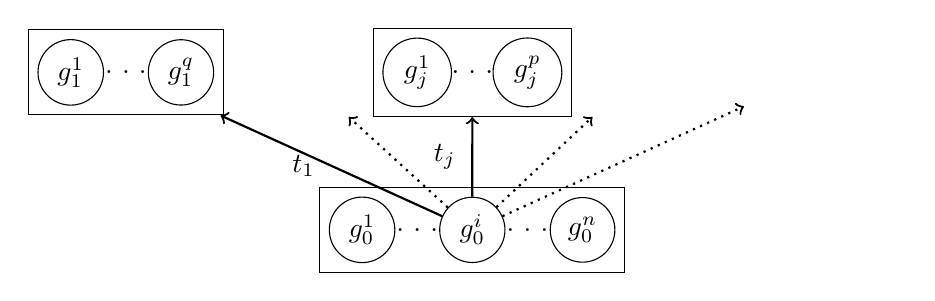
\begin{tikzpicture}[node distance=0.7cm]
\node [tcircle] (0) {$g_0^i$};
\node [right of=0] (0r) {.\ .\ .};
\node [tcircle,right of=0r] (0rr) {$g_0^n$};
\node [left of=0] (0l) {.\ .\ .};
\node [tcircle,left of=0l] (0ll) {$g_0^1$};
\node [draw,fit=(0rr) (0ll)] {}; 
\node [above of=0,node distance=2cm] (2) {.\ .\ .};
\node [left of=2, tcircle] (2l) {$g_j^1$};
\node [tcircle,right of=2] (2r) {$g_j^p$};
\node [draw, fit=(2l) (2r)] (2b) {}; 


\node [tcircle, left of=2l, node distance=3cm] (1r) {$g_1^q$};
\node [left of=1r] (1) {.\ .\ .};
\node [tcircle, left of=1] (1l) {$g_1^1$};
\node [draw, fit=(1l) (1r)] (1b) {}; 

\node [right of=2r,node distance=3cm] (3l) {$\phantom{g_3^p}$};
\node [right of=3l] (3) {\phantom{.\ .\ .}};
\node [right of=3] (3r) {$\phantom{g_3^p}$};
\node [fit=(3l) (3r)] (3b) {};

\node [fit=(1r) (2l)] (1m) {}; 
\node [fit=(2l) (3r)] (2m) {}; 

\draw[-to,thick] (0) to node[xshift=-10](t1){$t_1$} (1b);
\draw[-to,thick] (0) to node[xshift=-10](t2){$t_j$} (2b);
\draw[-to,dotted,thick] (0) to (1m);
\draw[-to,dotted,thick] (0) to (2m);
\draw[-to,dotted,thick] (0) to (3b);
\end{tikzpicture}
\end{center}
\caption{The two branching factors: choice of a goal $g_0^i$ and choice of a 
tactic $t_j$.}
\label{fig:choice}
\end{figure}

Starting from the bottom node, we can construct descendant of this node by 
choosing a goal $g_i^0$ on this node and choosing tactics $t1,t2,\ldots$ to 
apply to this goal. Here the result produces new nodes each containing a list 
of goals to be proven. 


Since there is a bijection between tactics of the tree search 
and the node they 
produced, any function define on tactics of the tree search can be map to a 
function defined on nodes. 


Supervised learning introduction.
\subsection{Prior tactic policy}

The estimation through the distance produced by the tactic selectors are hard 
to translate into a prior tactic policy, so we rely only on the order of 
tactics to estimate the probability with which a tactic should be tried.
Let $t_0,\ldots,t_500$ be the list of preselected tactics ordered by their 
distance to a goal $g$. Let $c_policy$ be a constant heuristic that estimates 
how likely a tactic $t_i$ is to prove the goal compared to the rest of the 
tactics $t_{i+1},\ldots,t_500$. We make the strong assumption that $c_policy$ 
is constant across the search. We can now calculate the prior policy by:

\[PriorPolicy(t_{i}) = (1 - c_policy)^{i} * c_policy\]

The first term of the multiplication is the probability that none of the better 
ranked tactic is selected. 

In fact, these probabilities are never used directly and only serves as a 
guidance to our deterministic node selection algorithm over many simulations.

\subsection{Prior node evaluation}

We now concentrate on defining a reasonable evaluation function that also 
influences node selection in MCTS. Essentially, we estimate how 
interesting is the list of goals of a tactic to determine if we should continue 
searching in this direction. Theoretically, an interesting list of goal is one 
that has the shortest proof, and we could measure the likelihood of being 
provable in a number of steps from previous proof search. However, this 
approach produces a lot of negatives\todo{TG: cite Hard Negative mining (cite 
Deep math)}. So to reduce this number, we limit 
ourselves to feature vectors tested during orthogonalization. We declare a list 
of goals l to be positive, noted $l \in Positive$, if it is has been 
produced by the winner of an orthogonalization competition. We extend the 
definition of a $distance$ to a list of goals by considering the union of the 
features of the goals. The set of the $r$ set of goals closest to a set of 
goal $l$ is noted $Neighbour(r,l)$. We can define the set of positives and 
negatives within a radius $r$ of a 
list of goals $l$ to be $Positive(r,l) = \lbrace m \in Neighbour(r,l)\ |\ m \in 
Positive \rbrace$.

During our experiments, we evaluate output goals in three different manners 
with the following functions:

\begin{align*}
PriorEvaluation_{none} (a_i) &= 0 \\
PriorEvaluation_{productive} (a_i) &= 1\\
PriorEvaluation_r (a_i) &= \frac{card\ Positive(r,a_i)}{r}\\
\end{align*}

For all evaluations functions, if a tactic is not productive then there is no 
output to evaluate, so the result is a failure and a reward of $0$ will be 
given for this node. The same thing happens if the node selected is already 
proven or a descendant of a proven goal. 
Experimentally, it is preferable not to 
filter proven (or descendants of proven) nodes before 
node selection to keep the estimation of the algorithm balanced.


\subsection{Node selection}

A similar trade-off between exploration and exploitation exists in algorithm 
like Monte Carlo. However, Monte Carlo tree search metrics are based on many 
simulations and do not reflect our exploration strategy that only 


We present here a monte carlo tree search with no roll out which is essentially 
the same as the one use by AlphaGo Zero~\cite{} originally defined by \cite{} 
in \cite{}.

\[Value(a_i) = Exploitation(a_i) + c_{exploration} * Exploration(a_i)\] 

The exploration term is determined by the prior policy and the current policy 
where as the exploitation is exactly the current evaluation build from prior of 
evaluations of descendants of $a_i$.



\[Exploration(a_i) = \frac{PriorPolicy(a_i)}{Policy(a_i)}\]

\[Policy(a_i) = \frac{1 + Visit(a_i))}{\sqrt{Visit(p))}}\]
The policy is approximatively the  percentage of time a node was visited.The 
square root skews this probability to favor even more exploration of nodes with 
few visits. 

The exploitation function $Exploitation$ is the average of the evaluation of 
all nodes descendant of $a_i$ (itself included) in the current search tree.   
\[Exploitation{a_i} = Average_{b \in Desc(a_i))} {PriorEvaluation(b)}\]


MCTS with prior policy
This modification of the search tree can be simulated by weighting each arrow 
by the distance shown by the diagonalized tree. To simulated the 
diagonalization in the original tree, the arrow $t_i$ will be given weight $i$.
Methods for exploring a tree with a large branching factor has been explored  
in Go~\cite{alphago} and 

However for very large branching factor RTS Combinatorial Multi-armed Bandits
for Real-Time Strategy Games. The method of choice for solving those 
problems 
is monte carlo tree search~\cite{mcts} which is a way to assign probabilities 
to each branches

In the context of changing wiehgts, the diagonalized tree has the advantage of 
being a little faster to explore as the ordered of tactic is inscribed in the 
shape of the tree. if the prior shapes 

\subsection{Node extension}

To prevent tactics from looping, we add timeout of 0.02 seconds to all tactics 
(optimized from previous paper)

\begin{definition} (Productive tactic)
During a proof search, after a tactic $t$ is applied to a node with active goal 
$g$, 
$t$ is called 
productive if and only if all the following conditions are satisified:
\begin{itemize}
\item It does not fail. We note $l$ the list of goals returned by the tactic.
\item It does not loop. $l$ do not contain any goals that appears in its 
ancestor nodes.
\item It is not a parallel step. $l$ is not a superset of a list of goals 
produced from the same node with the same active goal.
\end{itemize}

The third point of the definition is a partial attempt to prevent confluent 
branches. The general 
case where two branches becomes parallel after $n$ steps is handle by a
tactic cache which memorizes tactic effects on goals. Similarly there is also a 
prediction cache, which memorize the tactic predictions for each goal. Those 
two caches allow a fast exploration of confluent branches but they remain 
separated in our search tree.

\paragraph{Solving a goal and a node}
Describe the case where a proof for a goal in a node is found.
If one of those list where empty, the goal $g_i^0$ would 
be proved.
A node is solved when every of its goal are solved.


\subsection{End of the proof search}
The proof search stops when one of these 3 conditions is realized:
\begin{itemize}
\item It found a proof (i.e. the root node is solved). In this case, 
the search returns a minimized and 
prettified proof script (see Section~\ref{sec:proofdisplay}).
\item It has saturated. 
There is no more tactics to be applied to any open goal. \todo{define open 
goal}
\item It exceeded a given time limit.
\end{itemize}

The second case happens very rarely (less than 10 times when evaluating 7088 
theorems) and only at the beginning of the library when the learned dataset is 
small. So in our experiments, we just give the number of proof found relative 
to the number of proof attempts.



\end{definition}





\subsection{Evaluation} 




%A large difference between diagonalized search and our MCTS algorithm is in 
%what is considered to be the width of the tree. In diagonalized search, 
%non-productive tactics contribute to the extension of the width where as in 
%MCTSn the width includes only the total number of children produced. The 
%influence of non-productive on the proof exploration is recovered when we 
%include an 
%evaluation function that takes into account the productivity of tactics such 
%as 
%$E_{productive}$ or $E_r$.





%Obviously, we can consider the 
%trivial evaluation function where 
%a goal is given reward if and only if it is proven. Yet, to make this approach 
%effective would require to learn on a very large amount of relatively easy 
%problems. To lessen the requirement of an very large amount of data, we 
%propose 
%to use our goal distance to select the $k$ closest goals that were proven 
%before. The following formulas shows how we can combine positive examples and 
%negatives examples to evaluate an unseen 
%goals.
%
%%Hard Negative mining (cite Deep math)
%
%\[\mathfrak{N}_m=\lbrace g\ |\ (N(g) \wedge n(g) \geq m) \vee 
%(P(g) \wedge p(g) >  m)\rbrace\]
%\[\mathfrak{P}_m=\lbrace g\ |\ P(g) \wedge p(g) \leq m \rbrace\]
%
%
%\[E(m) = \frac{1}{m} \times \frac{card\ \mathfrak{P}_m}
%    {card\ \mathfrak{N}_m + card\ \mathfrak{P}_m} \]
%
%
%\[E = \argmax_{m \in \mathbb{N}} E(m)\]
% 

%We need
%MCTS.
%We use supervised learning to estimate evaluation functions.
%
%Positives are given the number of intermediate steps needed to finish the 
%proof.
%And the distance for negatives is two times the number of intermediate steps 
%tried. If we only tried one more tactic on this goal we would solve it.


%We use K-nn on them with k = 10 and calculate an the following weighted mean.
%
%
%The heuristic component should represent the number of steps (or total time) 
%estimated required to 
%solve the goal.
%If a goal is not provable then it's the number of time the goal was visited 
%during the search + 1.

%
%
%Combining with general automation:
%metis.
%holyhammer. (with orthogonalized theorems).
%divide by the sum of the weight of all features.
%
%
%New astar heuristic:
%The astar algorithm was simplified and now is represented in the standard 
%additive form instead of the multiplicative one described in our previous 
%paper.
%
%We also tried to estimate the difficulty of a goal. How likely that a 
%conjunction of goals are provable.
%
%Heuristic from prediction score:
%
%Heuristic from positives:
%
%Heuristic from positives + hard negatives.
%
%Admissibility of the heuristic:
%  
%Connection with UCB, UCT and Monte Carlo.
%
%Why is it not applicable in our case?
%
%1) Monte carlo requires to explore every action at least once. 
%This could be fixed by predicting fewer tactics 10-20. But we do not have
%yet an automatic way to tell.
%
%2) Monte Carlo requires a evaluation of the provability of the goal.
%This is insight can be gain.
%
%\subsection{Node selection formula}
%Monte Carlo tree search is a tree search algorithm. It explores the proof tree
%by performing simulation from the root to a leaf of the tree by selecting each 
%node by looking at that includes exploration and exploitation. Intuitively, 
%the 
%trade-off between exploitation and exploration means that the algorithm will 
%exploit deeper more promises branches but leaving enough time for exoloring 
%less likely alternatives.
%
%
%
%Connection with previous tree search. The prior probabilities are decreasing
%exponential of 2s. $\sqrt (n) > 1/2^n$
%
%
%
%
%
%calls simulation. 
%
%
%
%\subsection{Description of the evaluation function}
%
%Non local heuristic for evaluation. Should consider also what is needed to be 
%proven.
%
%
%In order to evaluate how long it takes to prove a goal. We collect data from 
%previous proof searches. Those include negative and positive examples.
%Positives examples are associated with the minimal number of steps needed to 
%find their proofs. Negative examples carry along the largest proof search 
%unsuccessfully performed.
%
%Combining this measure in an single evaluation of the proof length is a 
%challenging task. We use the following formulas P1 for estimating the 
%probability of being provable in less than one step.
%
%Neg(i) = not provable in i steps.
%70 percent change of not being provable in two steps.
%50 percent chance of closing the proof in 1 step: 2
%1 percent chance of being provable in 1 steps.
%20 percent chance of being provable in 2 steps. 5*2 = value = 10
%100 percent chance of being provable in 5 steps. 5
%
%\[P_i = Neg(i) | Knn(10) \] 
%
%the total estimation is given by:
%\[E = (\sum_{i=1}^5 (1-P_i)) + 1\] 
%
%\subsection{Combining evaluation function on goals}
%
%Independence of each probabilities.
%Full correlation: $(P1 * P2 * P3) ^{1/3}$
%Min probabiity:



%
%\subsection{Advantage of Monte Carlo Tree Search over A*-search}
%- Take into account all estimation along the proof and not only the last leaf.
%- Easy to link conjunction estimation   together.
- 

\section{ATP Integration}\todo{TG + JU + CK: rework and review}
General-purpose proof automation mechanisms which combine proof translation to
ATPs with machine learning (``hammers'') have become quite successful in
enhancing the automation level in proof assistants~\cite{hammers4qed}.
As external automated reasoning techniques sometimes outperform the combined 
power of tactics, we would like to combine the \tactictoe search with 
stronger general purpose provers such as the one in \holyhammer for 
\holfour~\cite{tgck-cpp15}. 

During our experiments,
We chose to distinguish two these general purpose tactic \metis and \eprover.
\metis is integrated in \holfour, so can be call with frequently with low 
timeout.
And the strongest external provers according to past experiments \cite{hh4h4}.
Where as...
external calls to \eprover are computationally expensive (5 seconds at a 
minimum +  128 premises), we  
experiment with a small hammer tactic comprised of: a faster premise 
selection algorithm and
a short call (0.1 seconds + 16 premises optimized by the previous paper) to the 
internal prover \metis~\cite{metis} or a
longer call to external prover \eprover. 



\paragraph{Prediction of general purpose tactics}
Since we do not always have the data to learn on which goal this general 
tactics are successful, we assume as a first approximation that they are the 
strongest all around. 

And we try them first on each node during the proof search with the advantage 
that if it succeeds the node is closed rapidly.

This general tactics requires a list of relevant lemmas.

This forced behavior could often be rediscovered from the training data for the 
internal provers \metis by using theorem abstraction. essentially a call to 
\metis where its 
theorem list argument has been abstracted.


\paragraph{Application of general purpose tactics}
The slightly higher timeout of 0.1 seconds given to \metis does not slowdown 
the proof too much but...
To integrate a general tactic that requires a higher time out such as \eprover, 
we make use of asynchronous calls via PolyML.fork to prevent the ATP 
from slowing down the search. 

%The number of parallel threads can be capped.
%And if tactictoe or an asynchronous thread proves a goal, all descendants of 
%these goal are deactivated, terminating associated threads. This frees space 
%for more pending threads, associated to newly created nodes, to start.


%needs to be taken after each proof step to close proofs solved by \eprover
%When the number of thread reaches a limit, a ``hammer'' tactic call 
%should
%wait for a thread to be freed but the proof search goes on and the feedback of 
%the ``hammer'' tactic is delayed. 
%
%
%It is best tactic available but we do not have any data about it since it does 
%not appear in any proofs. So , we 
%artificially try it on

%\paragraph{Effect on orthogonalization of tactics}
%During orthogonalization, the general purpose tactic will be the first 
%competitor and if it manages to prove the goal it will subsume the original 
%tactic on this goal since the empty set of goals is a subset of any set. 
%Therefore, it will replace the original tactic in the feature vector that is 
%competed for. This is desirable since we would like to remove alternative 
%proofs.

%\paragraph{Orthogonalization of theorems}
%A ``hammer'' tactic can be useful to remove parallel
%theorems. We consider a theorem to be parallel if it can be proven 
%from previous theorems using a general tactic with a timeout equal or less 
%than the one it is given during the proof search. Parallel theorems are marked 
%and removed from the set of theorems $\mathfrak{T}$ from 
%which premise selection is performed.
%
%\begin{remark}
%The ``smaller hammer'' is chosen to remove parallel theorems and as the first 
%try during orthogonalization of tactics. 
%\end{remark}


%\paragraph{Effect on the proof search}
%First, before the proof search, we preselect 500 theorems 
%for the whole proof search tree using a premise selection algorithm 
%that takes into account dependencies between theorems.
%During the proof search, when a new goal is created or a fresh pending goal is 
%considered, the ``hammer'' tactic is always tried first because if it succeeds 
%the node would be closed rapidly.

%\paragraph{Parallelization of external calls}
%It is possible to parallelize calls to external provers so that they happen 
%asynchronously during the proof search. We let the prover runs \tactictoe 
%continue its proof in parallel of a ``hammer'' tactic call.


\section{Experimental Evaluation}\label{s:experiments}\todo{TG: introduction + 
consistent tables}

Disclaimer:
Conditions of the experiments may vary slightly between different tables 
because of various factors such 
as overhead cost of additional features or the fact that they were run on 
different machines on a local machine or on the server.

\subsection{Methodology} \todo{TG: is copied, update references of sections and
new algorithm + mention when orthogonalization is done}

The evaluation imitates the construction of the library: For each theorem only 
the previous human proofs are known. These are used as the learning base for 
the predictions.
To achieve this scenario we re-prove all theorems during a modified build of 
\holfour.
As theorems are proved, their tactical proofs and their statements are recorded 
and included in the 
training examples.
For each theorem we first attempt to run the \tactictoe search with a time 
limit of 5 seconds,
before processing the original proof script.
In this way, the fairness of the
experiments is guaranteed by construction. 
Only previously declared \sml 
variables (essentially tactics, theorems and simpsets) are accessible. 
And for each theorem to be re-proven \tactictoe is only trained on previous 
proofs.



\paragraph{Dataset}

All top-level theorems in the standard library are considered except:
\begin{itemize}
\item the 619 calls to store\_thm that contains a let binding, these are 
typically 
harder for \tactictoe as it may not have seen the particular local declaration 
before and therefore would have to find an alternative proofs. We also do not 
learn from these proofs because they were explictly local.
\item the 1175 calls to save\_thm. These are typically mostly trivial and easy 
theorems.
The remaining 7088 top-level theorems are evaluated in the full scale 
evaluation and the level of difficulty of these problem is assessed by a 
comparison with \eprover.
\end{itemize}

Among these types of theorems, every tenth theorems of the first third of the 
library is evaluated during tuning, which give us a total of 273 theorems to 
train different parameters on.

\paragraph{Strategy selection}
Although the training process in each strategy on its own is fair, the 
selection of the 
best strategy in Section~\ref{sec:sel_param} should also be considered as a 
learning 
process. To ensure the global fairness, the final experiments in 
Section~\ref{sec:exp_full} 
runs the best strategy on the full dataset which is about 10 times larger. The
performance is minimally better on this validation set.

\subsection{Tuning \tactictoe}

\subsubsection{Prediction parameters}\todo{TG: remove this section or mention
that parameters were optimized in the previous version}
The first experiment concerns the choice of the right kind of features and 
feature scoring 
mechanism. The results are presented in Table~\ref{tab:feature_param}.
We observe that the higher-order features and the feature of the top logical 
structure increase minimally the number of problems solved. The attempted 
length penalty on the total number of features is actually slightly harmful.
We did not turn on the top feature flag in the next experiments because they 
are slightly more expensive too compute.

%
%\begin{table}[t]
%\centering\ra{1.3}
%\small
%\begin{tabular}{llll}
%\toprule
% ID & Learning parameter & Solved & $U(D_1)$ \\
%\midrule
% $D_0$ & $codist_1$ (length penalty) & 172 (20.0\%) & 5 \\
% $D_1$ & $codist_0$ (default) & 179 (20.8\%) & 0 \\
% $D_2$ & no top features & 175 (20.3\%) & 18 \\
% $D_3$ & no higher-order features & 178 (20.7\%) & 8 \\
%\bottomrule
%\end{tabular}
%\caption{\label{tab:feature_param}Success rate of strategies with different 
%learning parameters on the training set.}
%\end{table}
%
%\subsubsection{Search parameters}
%
%\paragraph{tactic timeout}
%\begin{table}[t]
%\centering\ra{1.3}
%\small
%\begin{tabular}{llll}
%\toprule
% ID & Searching parameter & Solved & $U(D_{9})$ \\
%\midrule
% $D_1$ & $codist_0$ (default)      & 179 (20.8\%) & 10 \\
% $D_4$ & tactic timeout 0.004 sec & 175 (20.3\%) & 9 \\
% $D_5$ & tactic timeout 0.1 sec   & 178 (20.7\%) & 10 \\
%\bottomrule
%\end{tabular}
% \caption{\label{tab:search_param}Success rate of strategies with different 
% search parameters on the training set.}
%\end{table}

\subsubsection{MCTS parameters: policy and evaluation}

\begin{table}[ht]
\centering\ra{1.3}
\small
\begin{tabular}{llllll}
\toprule
 $c_{policy}$ & Width & Ortho & Eval & $c_{exploration}$ & Solved \\
\midrule
 2/3 & All & No & $E_{none}$ & 1 & 120\\
 1/2 & All & No & $E_{none}$ & 1 & 125\\
% 1/2 & All & Yes & $E_{none}$ & 1 & 130 \\
 1/3 & All & No & $E_{none}$ & 1 & 117\\
% 1/2 & Productive & No & $E_{none}$ & 1 & 120\\
% 1/2 & Productive & No & $E_{productive}$ & 1 & 127\\
\bottomrule
\end{tabular}
\caption{\label{tab:cost_param} on a local machine}
\end{table}

%This experiments were performed without the square root in the policy 
%function.

\begin{table}[ht]
\centering\ra{1.3}
\small
\begin{tabular}{llllll}
\toprule
  $c_{policy}$ & Width & Ortho & Eval & $c_{exploration}$ & Solved \\
\midrule
 1/2 & All & No & $E_{none}$ & 1 & 122\\
 1/2 & All & Yes & $E_{none}$ & 1 & 128\\
 1/2 & Productive & Yes & $E_{none}$ & 1 & 128\\
 1/2 & Productive & Yes & $E_{productive}$ & 1 & 134\\ 
 &  & &  & 4 & 130\\
 1/2 & Productive & Yes & $E_1$ & 1 & 127\\ 
 & & & & 4 & 126\\ 
 1/2 & Productive & Yes & $E_{10}$ & 1 & 136\\ 
 & & & & 4 & 137\\ 
\bottomrule
\end{tabular}
\caption{\label{tab:learning} on the server}
\end{table}

We settled for the first parameters where an evaluation function based on 
machine learning was beneficial. It is highly likely than better parameters for 
the policy, radius of evaluation and exploration coefficient can be found with 
further investigation.

%\begin{table}[ht]
%\centering\ra{1.3}
%\small
%\begin{tabular}{ll}
%\toprule
% & Solved \\
%\midrule
% diag coeff: 0.5 & 120\\
% diag coeff: 1   & 125\\
% diag coeff: 1 + orthogonalization & 130 \\
% diag coeff: 2 &  117\\
% no evaluation & 120\\
% trivial evaluation E1 & 127\\
%\bottomrule
%\end{tabular}
%\caption{\label{tab:cost_param} on a local machine}
%\end{table}
%
%\begin{table}[ht]
%\centering\ra{1.3}
%\small
%\begin{tabular}{ll}
%\toprule
% & Solved \\
%\midrule
% none & 122\\
% ortho & 129\\
% no evaluation + ortho & 128\\
% trivial evaluation + ortho    & E1:134 E4:130\\
% evaluation radius: 1 + ortho  & E1:127 E4:126\\
% evaluation radius: 10 + ortho & E1:136 E4:137\\
%\bottomrule
%\end{tabular}
%\caption{\label{tab:learning} on the server}
%\end{table}


We preselect around each feature vectors, one hundred feature of but this takes 
time. What kills us is the time needed to select the neighbors among the 
maximum of 50,000 feature vectors but maybe we can hope to 
taking half the time of the proof search.


\subsection{Increasing \tactictoe's knowledge}\label{sec:perfect_exp}

We investigate what are the limits of \tactictoe and what benefits additional 
knowledge could provide. To this end, we will modify the set of features to 
include features vectors that should not be known in a regular experiment. We  
include some vectors from the recorded human proof and perform the proof search 
after the recording instead of before in all other experiments. This experiment 
is not fair and should only be compared to 
experiments in the same settings.

For clarity, we will name the set of feature vectors that can be recorded from 
the current human proof $\mathbb{H}$ and the set of vectors recorded from 
previous proofs $\mathbb{P}$ (consistent with previous notation?). We note 
$\pi_1^1$ the projection on the 
first component returning the label of a feature vector. And we define the 
function $T$ that takes a tactic and return the list of its tokens.

We will progressively add bigger and bigger 
subset of $\mathbb{H}$ to $\mathbb{P}$ and observe the effect on the proof 
search success rates. 

Here are the list of increasing non-trivial subsets of $\mathbb{H}$ we consider:
\begin{align*}
\mathbb{F}_1 &= \lbrace (t,g) \in \mathbb{H}\ |\ t \in \pi_1^1(\mathbb{P})  
   \rbrace \\
\mathbb{F}_2 &= \lbrace (t,g) \in \mathbb{H}\ |\ \forall x \in T(t).\ \exists 
t'\in \pi_1^1(\mathbb{P}).\ x \in T(t') \rbrace\\
\mathbb{F}_3 &= \lbrace (t,g) \in \mathbb{H}\ |\ \forall x \in T(t).\ \exists 
t'\in \pi_1^1(\mathbb{P}).\ x \in T(t') \vee x\ \mbox{is a theorem} \rbrace\\
\mathbb{F}_4 &= \lbrace (t,g) \in \mathbb{H}\ |\ \forall x \in T(t).\ \exists 
t'\in \pi_1^1(\mathbb{P}).\ x \in T(t') \vee x\ \mbox{is a theorem or a term} 
\rbrace\\
\end{align*}


$\mathbb{F}_1$ is an approximation of what we could get if we had perfect 
prediction for those tactics.


\begin{table}[h]
\centering\ra{1.3}
\small
\begin{tabular}{lll}
\toprule
 & Additional features & Solved \\
\midrule
$\emptyset$ & none & 119 (43.6\%) \\ %NONEv2
$\mathbb{F}_1$& tactic prediction & 121 (44.3\%) \\ %AFTERTACv2
$\mathbb{F}_2$& token recombination  & 137 (50.2\%) \\ %AFTERTOKENv2
$\mathbb{F}_3$& theorem prediction  & 207 (75.8\%) \\ %AFTERTHMTHMv2
$\mathbb{F}_4$& term prediction & 223 (81.7\%) \\ %AFTERALLv2
$\mathbb{H}$     & all & 239 (87.5\%) \\ %AFTERSMALLv2
% $AFTERv2$       & $\mathfrak{H}$ & 245 (89.7\%)  \\
\bottomrule
\end{tabular}
\caption{\label{tab:featue_param} Success rates of with an artificially 
augmented dataset of features fetched from the human proof of the tested 
theorem}
\end{table}

And we observe in Table~\ref{tab:featue_param} a 
slight increase compared to the default \tactictoe. We then included all 
vectors that contains tactics that can be rebuild from tokens of
tactics in our database. 
Our search algorithm proved two proofs less that if it had perfect prediction 
so it means that our prediction algorithm (policy) is doing a good  job at 
least in this early settings where proofs are easy. 
Suprisingly, being able to recombine tokens of tactics from the database is 
barely sufficient to prove more than half of the theorems in this dataset. The 
Therefore, additionally including in tactics theorems and terms that did not 
appear in previous tactics is essential. Creating from scratch other arguments 
may not help as much. This is why we restricted ourselves to predicting 
arguments of theorem list type and the term type during tactic synthesis. 
Finally our proof search algorithm sometimes fails even if it knows all the 
tactic necessary. The two main reasons are that either a crucial tactic exceeds 
its timeout or that the human proof is too deep to be rediscovered (more than 
10 steps long).

\subsubsection{Abstraction}
Here, we test the benefit of different kind of tactic abstraction. 
In all those experiments orthogonalization is performed with radius 20 but not 
orthogonalization with respect to metis.


All experiments in this table are using orthogonalization.
\begin{table}[t]
\centering\ra{1.3}
\small
\begin{tabular}{ll}
\toprule
  & Solved \\
\midrule
% holyhammer & 79 \\
 none & 122\\
 ortho & 129\\
 ortho + term & 126\\    
 ortho + theorem list & 160\\
 ortho + metis & 162\\
 %ortho + metis + thmortho & 155\\
 %ortho + metis + stacortho & 160\\
 ortho + metis + theorem list & 175\\ 
\bottomrule
\end{tabular}
\caption{\label{tab:cfot_param}
Sucess rates of tactictoe with synthesis for different arguments.}
\end{table}
We want to know what the optimal number of predictions for tactics different 
from \metis since \metis has a special status in our algorithm is handled 
independently.

\subsubsection{ATP integration}

%The third experiment, presented in Table~\ref{tab:lh_param},
%evaluates the effect of integrating the ``small hammer'' in the \tactictoe 
%search.
%At a first glance, the increased success rate is significant for all tested 
%parameters. 
%Further analysis reveals that increasing the number of premises from 8 to 16 
%with a 
%timeout of 0.02 seconds is detrimental. The $D_{19}$ experiment  demonstrates 
%that 0.1 
%seconds is a better time limit for reasoning with 16 premises. And the 
%$D_{18}$ 
%experiment reveals the disadvantage of unnecessarily increasing the timeout of 
%\metis. This reduces the time available for the rest of the proof search, 
%which 
%makes the success rate drop.

The best setting for \metis was to be in previous experiments to be 16
theorems and


%\begin{table*}[t]
%\centering\ra{1.3}
%\small
%\begin{tabular}{llll}
%\toprule
% ID & ``small hammer'' parameter & Solved &  $U(D_{19})$ \\
%\midrule
% $D_9$ & $codist_5(0.8,0.8)$ (default: no small hammer) & 211 (24.5\%) & 19 \\
% $D_{16}$ & 8 premises + timeout 0.02 sec & 281 (32.7\%) & 21 \\ 
% $D_{17}$ & 16 premises + timeout 0.02 sec & 270 (31.4\%) & 18 \\
% $D_{18}$ & 8 premises + timeout 0.1 sec & 280 (32.6\%) & 11 \\
% $D_{19}$ & 16 premises + timeout 0.1 sec & 289 (33.6\%) & 0 \\
%\bottomrule
%\end{tabular}
% \caption{\label{tab:lh_param}Success rate of strategies with different 
% parameters of
% ``small hammer'' on the training set.}
%\end{table*}

The best strategy which does not rely on the ``small hammer'' approach $D_9$ 
will be called \tactictoe(NH) (for no ``small hammer'') in the remaining part 
of the paper, and the best strategy relying on the approach, $D_{19}$, will be 
referred to as \tactictoe(SH) (``small hammer'').

%\begin{table}[h!]
%\centering\ra{1.3}
%\small
%\begin{tabular}{lll}
%\toprule
% ID & Orthogonalization of theorems & Solved \\
%\midrule
% $NONE$           &                             & 118\\
% $METIS16$        & using metis                 & 143\\
% $METIS16_NEW$    & no theorems from boolTheory & 155\\
% $METIS16v2NOINT$ & no internal theorems        & 159\\
% $METIS16v2DIAG$  & diagonal exploration        & 166\\ 
% $METIS16v2INT$   & internal theorems           & 168\\
% $METIS16_30$     & 30 seconds timeout          & 162\\
%\bottomrule
%\end{tabular}
%\caption{\label{tab:cst_param}}
%\end{table}

\begin{table}[h!]
\centering\ra{1.3}
\small
\begin{tabular}{ll}
\toprule
  & Solved \\
\midrule
   \eprover &  106 \\
   \tactictoe &  139 \\
   \tactictoe + \metis & 182 \\
   \tactictoe + asynchronous \eprover & 182 \\
%x tactictoe + async holyhammer 10 & 183 \\
   \tactictoe + \metis + asynchronous \eprover & 190 \\
  
\bottomrule
\end{tabular}
\caption{Experiments with a timeout of 60 seconds \label{tab:param}}
\end{table}

\subsection{Full-scale experiment}

Mention the conflicts.
Theorem orthogonalization is not turn on during instantiation of tacitcs except 
for the metis tactic.
Best parameters + comparison with holyhammer.




Until now, all our feature vectors were learned form human proofs. 
human proofs. We can also add to this tactics that were part of a proof found 
by our algorithm. To prevent duplication of effort, orthogonalization of those 
tactics is essential to have a beneficial effect (see Experiments).
Since recording and re-proving are intertwined, the 
additional data is available for the next proof search.
The hope is that the algorithm will improve faster by learning from its own 
discovered proofs than from the human proof 
scripts~\cite{DBLP:conf/cade/Urban07}. It is also the first step toward 
self-reinforcement learning.





\begin{table}[h!]
\centering\ra{1.3}
\small
\begin{tabular}{llll}
\toprule
  & & Small(273) & Big(7088) \\
\midrule
  & \eprover (auto-schedule + 128 premises) & 86 & 2069 (29.19\%)\\ 
%  & \tactictoe (without special care for metis) & 154 & 3868 (\\
  & \tactictoe (best parameters) & 187 & 4186 (59.06\%) \\
%  & \tactictoe (+ self-learning) & 187 (187) &  4201 (59.27\%) \\
\bottomrule
\end{tabular}
\caption{Experiments with a timeout of 10 seconds \label{tab:_param}}
\end{table}

It is learning to use \metis however it cannot automatically learn to give it 
more time making it still a bit weaker than the adhoc startegy.



Table~\ref{theories} compares the success rates of re-proving for different
\holfour theories. \tactictoe(SH) outperforms \tactictoe(NH) on every 
considered theory.
Even if a lot weaker due to the missing premise selection component, 
\tactictoe(NH)
is hugely better than \holyhammer(blistr) in 4 theories: \texttt{measure}, 
\texttt{list}, \texttt{sorting} and \texttt{finite\_map}. The main reason is 
that 
those theories are equipped with specialized tactics, performing complex 
transformation such as structural induction and \tactictoe(NH) can reuse them. 
Conversely, \holyhammer(blistr) is more suited to deal with dense theories such 
as 
\texttt{real} or \texttt{complex} where a lot of related theorems are available 
and 
most proofs are usually completed by rewriting tactics.

\begin{table}[]
\centering
\setlength{\tabcolsep}{3mm}
\begin{tabular}{@{}ccccc@{}}
\toprule
\phantom{ab} & {arith} & {real} & {compl} 
& {meas} \\
\midrule
\tactictoe & 74.6 & 67.3 & 77.3 & 28.2\\
\eprover & 50.8 & 67.6 & 63.4 & 10.8 \\
\midrule
\phantom{abc}  & {proba} & {list} & {sort} & {f\_map} \\
\midrule
\tactictoe & 37.3 & 71.4 & 58.4 & 73.6 \\
\eprover & 19.3 & 20.7 & 15.8 & 20.9 \\
\bottomrule
\end{tabular}
\caption{\label{theories}Percentage (\%) of re-proved theorems in the theories 
\texttt{arithmetic}, \texttt{real}, \texttt{complex}, \texttt{measure},  
\texttt{probability}, \texttt{list}, \texttt{sorting} and \texttt{finite\_map}. 
}
\end{table}  


\subsection{Time and space complexity}

Analysing failed proof attempt can give us an idea of the behaviour of the 
algorithm. In a proof search of 10 seconds, in average 500 (todo: real 
estimation) tactics are applied.
The productive tactics create an average of 100 (todo: real estimation) nodes. 
This means that in this settings 1 out of 5 tactics are productive.

Increasing the timeout to more than 10 seconds would probably be beneficial as 
we can see that the slope of the curve is far for being flat in Fig~..

\pgfplotscreateplotcyclelist{my black}{
solid, mark repeat=100, mark phase=0, black!100\\
dashed, mark repeat=100, mark phase=0, black!100\\
}

\begin{figure}[h]
\centering           
\begin{tikzpicture}[scale=1]
\begin{axis}[
  legend style={anchor=south east, at={(0.9,0.1)}},
  width=\textwidth,
  height=0.7*\textwidth,xmin=0, xmax=10,
  ymin=0, ymax=4500,
  xtick={},
  ytick={},
  cycle list name=my black]
\addplot table[x=time, y=solved] {data/tt_ptime};
\addplot table[x=time, y=solved] {data/e_ptime};
\legend{\tactictoe,\eprover}
\end{axis}
\end{tikzpicture}
\caption{Number of problem solved in less than x seconds.}
\end{figure}

\begin{figure}[h]
\centering           
\begin{tikzpicture}[scale=1]
\begin{axis}[
  legend style={anchor=north east, at={(0.9,0.9)}},
  width=\textwidth,
  height=0.7*\textwidth,xmin=0, xmax=10,
  ymin=0, ymax=100,
  xtick={},
  ytick={},
  cycle list name=my black]
\addplot table[x=size, y=solved] {data/tt_percent};
\addplot table[x=size, y=solved] {data/e_percent};
\legend{\tactictoe,\eprover}
\end{axis}
\end{tikzpicture}
\caption{Percentage of problem solved with respect to the length of the 
original 
proof}
\end{figure}

%\begin{table*}[t]
%\centering\ra{1.3}
%\small
%\begin{tabular}{llllll}
%\toprule
% ID & \multicolumn{2}{c}{nodes}   & \multicolumn{2}{c}{proof size} & 
% \multicolumn{1}{c}{time}\\ \cmidrule(lr){2-3} \cmidrule(lr){4-5} 
% \cmidrule(lr){6-6}
%     & average & max & average & max & average \\
%\midrule
% \tactictoe & 94.66 & 421 & 3.34 & 39 & 0.66 \\
%\bottomrule
%\end{tabular}
% \caption{\label{tab:stats} old search statistics}
%\end{table*}

Constant progress: 
  From 45 percent on the same dataset in 5 seconds 
       59 percent in december in 10 seconds
  Probably 65-70 percent en of January in 60 seconds.      

The progress cannot be attributed only to the time increase but to testing and 
debugging of parameters.

\section{Proof Presentation}\label{sec:proofdisplay}\todo{MN + RK: add 
motivations and transitions}

Motivation: 
+ minimal effort to integrate the tactictoe results in proof scripts.

Side effect:
+ could be also used to simplify existing proof scripts. 

\paragraph{Reconstruction}
When a proof search succeeds (there are no more pending goals at the root)
we need to reconstruct a \holfour human-style proof.
The saved nodes consist of a set of trees where each edge is a tactic and
the proof tree is the one starting at the root.
In order to obtain a single \holfour proof, we need to combine the tactics
gathered in the trees using tacticals.
By the design of the search, a single tactic combinator, \texttt{THENL}, is 
sufficient. It combines a tactic with a list of subsequent ones, in such a way 
that after the parent tactic is called, for each created goal a respective 
tactic from the list is called.
The proof tree is transformed into a final single proof script
 by the following recursive function $P$ taking a
tree node $t$ and returning a string:
\begin{equation*}
P(t) =
\begin{cases}
P(c) & \text{if $t$ is a root},\\
tac & \text{if $t$ is a leaf},\\
tac\ \texttt{THENL}\ [P(c_0),\ldots,P(c_n)] & \text{otherwise.}
\end{cases}
\end{equation*}
where $tac$ is the tactic that produced the node, $c$ is the
only successful child of the root and $c_0, \ldots, c_n$ are the 
children of the node produced by the successful tactic.

The readability of the created proof scripts is improved, by replacing
replacing  \texttt{THENL} by \texttt{THEN} when the list has length 1.
Further post-processing such as
removing unnecessary tactics and theorems has been developed and
improve the user experience greatly~\cite{DBLP:conf/sefm/Adams15}.

\paragraph{Minimizing length and time of the proof} 
First a weak minimization is possible when processing the final proof. If the 
tactic \texttt{A THEN B} appears in the proof and has the same effect as 
\texttt{B} then we can drop \texttt{A} from the proof.
Stronger minimization can be obtained by rerunning the prover with feature 
vectors containing only tactics 
from the proof. To obtain a shorter proof, the exploration coefficient should be
increased and the policy coefficient lowered to encourage exploration in the 
width of the proof tree. Additionally, by giving a weaker evaluation to slow 
tactics, we can aim for faster proofs.

\paragraph{Minimizing tactic arguments}
One of the argument that may contain unnecessary information are lists.
Let $t$ be a tactic applied to a goal $g$ containing a list $l$ as argument. 
And let $t'$ be the tactic $t$ where one element $e$ of $l$ as be removed. If 
$t$ and $t'$ have the same effect on $g$ then $t'$ can replace $t$ in the final 
proof.

This is a generalization of the simplest method used for minimizing a list of 
theorems in ``hammers'' \cite{}. The fact that lists are generally small
make this approach feasible.

\paragraph{Prettification}
Without prettification, the returned tactic is barely readable as it contains 
information to guarantees that each \sml subterm is interpreted in the way in 
any context. Our approach here is to strip this information from the tactic and 
test if the tactic has the same effect as the original one to guarantee that we 
are not changing the proof. For efficiency, 
this is performed on each tactic step separately. We strip module prefixes, 
local declaration. If local declaration can't be 
stripped, we try to group all local declarations under a single "let" binding 
which improves readability and prevents duplication of this declarations.


%\paragraph{Step by step exploration.}
%Because a human may have better insight on which tactic to chose next, we also 
%provides an interactive mode, where the user is presented the best $n$ 
%predicted tactics for a goal and to be chosen from. The number $n$ is 
%parameter 
%that can be chosen by the user. Those tactics are curated so that only 
%productive tactics are returned. (define productive)







\section{Case study}\todo{
  TG + RK: describe the two examples.
  RK: After implementation and small experiment is done (in about 1 week) 
      Test tactictoe find new examples on new goals and manual exploration mode.
      Give feedback.
}
%Investigating further the different qualities of \tactictoe, we study its 
%generated proof scripts on an example in \texttt{list} theory (see 
%Example~\ref{ex:casestudy}). 
%The theorem to be proven states the equivalence 
%between the fact that a number $n$ is greater than the length of a list 
%$\mathit{ls}$ with the 
%fact that dropping $n$ elements from this list returns an empty list.
%
%The human proof proceeds by induction on $n$ followed by solving both goals 
%using rewrite steps combined with an arithmetic decision procedure. 
%Both \tactictoe proofs (NH and SH) follow the general idea of reasoning by 
%induction but solve 
%the base case and the inductive case in a different way.
%The base case only needs rewriting using the global simpset in the 
%\tactictoe(NH)
%proof, which is simulated by a call to \metis in the (SH) proof.
%The inductive case should require an arithmetic decision procedure as hinted 
%by 
%the human 
%proof. This is achieved by rewriting using an arithmetic simpset in the second 
%proof. In the first proof however, a rewriting step and case splitting step 
%were used
%to arrive at a point where \metis calls succeed.
%The tactic proof produced by \tactictoe(NH) often looks better than the one 
%discovered by \tactictoe(SH) in that it does not involve \metis calls with a 
%large numbers of premises. 

%In general, \tactictoe does not search for beauty, but sometimes it is 
%discovered by accident.


%The term and the conversion rules were not synthesized but simply copied from 
%previous 
%proofs.

%Name: 218 SURJ_INJ_INV
%Original proof time: 0.002033

%SURJ_INJ_INV
%proof length: 2
%proof time: 0.050853
%Statistics
%  infstep : 31
%  nodes   : 11
%  maxdepth: 3
%Time: 1.300789
%  inferstep time: 1.071869
%  node_find time: 0.018046
%  node_crea time: 0.147604
%    pred time: 0.04263
%    thmpred time: 0.000005
%    mc time: 0.071282
%    inst time: 0.0
%Proof found: 
%Org tac number: 15
%Replaying proof: 0.562829




%\begin{remark}
%The additional difficulty produced by the necessary induction is such that the 
%theorem could not be proven by \holyhammer.
%\end{remark}

\newcommand{\wed}{\begin{math}\wedge\end{math}}

Proofs discovered by \tactictoe discovered during evaluation.




for theorem \texttt{SURJ\_INJ\_INV} In 
theory \texttt{pred\_set})



\begin{example}\label{ex:casestudy}()



%val SURJ_INJ_INV = store_thm(
%  "SURJ_INJ_INV",
%  ``SURJ f s t ==> ?g. INJ g t s /\ !y. y IN t ==> (f (g y) = y)``,
\vspace{5mm}
\small


Goal
\begin{lstlisting}[language=SMLSmall,frame=tb]
!f s t. SURJ f s t ==> ?g. INJ g t s wedge !y. y IN t ==> (f (g y) = y)
\end{lstlisting}

Original \holfour proof script (2.03 milliseconds)
\begin{lstlisting}[language=SMLSmall,frame=tb]
REWRITE_TAC [IMAGE_SURJ] THEN
  DISCH_TAC THEN Q.EXISTS_TAC `THE o LINV_OPT f s` THEN
  BasicProvers.VAR_EQ_TAC THEN REPEAT STRIP_TAC
  THENL [
  irule INJ_COMPOSE THEN Q.EXISTS_TAC `IMAGE SOME s` THEN
    REWRITE_TAC [INJ_LINV_OPT_IMAGE] THEN REWRITE_TAC [INJ_DEF, IN_IMAGE] THEN
    REPEAT STRIP_TAC THEN REPEAT BasicProvers.VAR_EQ_TAC THEN
    FULL_SIMP_TAC std_ss [THE_DEF],
  ASM_REWRITE_TAC [LINV_OPT_def, o_THM, THE_DEF] THEN
    RULE_ASSUM_TAC (Ho_Rewrite.REWRITE_RULE
      [IN_IMAGE', GSYM SELECT_THM, BETA_THM]) THEN ASM_REWRITE_TAC [] ]
\end{lstlisting}

\vspace{5mm}

\tactictoe proof script (50.85 milliseconds)
\begin{lstlisting}[language=SMLSmall,frame=tb]
SRW_TAC [] [SURJ_DEF, INJ_DEF] THEN METIS_TAC []
\end{lstlisting}




Goal
\begin{lstlisting}[language=SMLSmall,frame=tb]
!l1 l2 n x. LENGTH l1 <= n ==> 
  (LUPDATE x n (l1 ++ l2) = l1 ++ (LUPDATE x (n - LENGTH l1) l2))
\end{lstlisting}

\vspace{5mm}

Original \holfour proof script (62.69 milliseconds)
\begin{lstlisting}[language=SMLSmall,frame=tb]
  rw[] THEN simp[LIST_EQ_REWRITE] THEN Q.X_GEN_TAC `z` THEN
  simp[EL_LUPDATE] THEN rw[] THEN simp[EL_APPEND2,EL_LUPDATE] THEN
  fs[] THEN Cases_on `z < LENGTH l1` THEN
  fs[] THEN simp[EL_APPEND1,EL_APPEND2,EL_LUPDATE]
\end{lstlisting}

%Name: 224 LUPDATE_APPEND2
%Original proof time: 



%val LUPDATE_APPEND2 = Q.store_thm("LUPDATE_APPEND2",
%   `!l1 l2 n x.
%      LENGTH l1 <= n ==>
%      (LUPDATE x n (l1 ++ l2) = l1 ++ (LUPDATE x (n-LENGTH l1) l2))`,
%);
\vspace{5mm}

\tactictoe proof script (17.16 milliseconds)
\begin{lstlisting}[language=SMLSmall,frame=tb]
Induct_on `l1` THENL [SRW_TAC [] [],
  Cases_on `n` THENL [SRW_TAC [] [],
    FULL_SIMP_TAC (srw_ss ()) [] THEN METIS_TAC [LUPDATE_def]]]
\end{lstlisting}


If a discovered proof is reasonable short, fast, maintainable  and 
understandable, they could 
replace its original in the \holfour standard library. In the first case the 
tactictoe proof is slower but could still be considered becaues it is much more 
readable. In the second case, it is faster and more readable.



%
%LUPDATE_APPEND2
%proof length: 6
%proof time: 0.017156
%Statistics
%  infstep : 70
%  nodes   : 27
%  maxdepth: 4
%Time: 3.02716
%  inferstep time: 2.12842
%  node_find time: 0.07146
%  node_crea time: 0.508384
%    pred time: 0.164047
%    thmpred time: 0.000012
%    mc time: 0.265314
%    inst time: 0.0
%Proof found: 
%Org tac number: 10
%Original proof time: 0.0
%Replaying proof: 0.470118






\end{example}

\section{Conclusion}\label{sec:concl}\todo{TG + JU or CK review}

Future work:
  Promising techniques that could not be evaluated. 
  + Orthogonalization of theorems~\cite{ckju-jsc15}. 
  + Try harder and smarted on term predictions. \cite{latest version of sepia}. 
  \cite{conjecturing}
 
More training than just orthogonalization of tactics.

%A first successful use of orthogonalization techniques for theorems appeared in
%a work on lemma mining~\cite{ckju-jsc15} in \hollight. Theorems were mined 
%from 
%proofs recorded at the kernel level. Because the number of recorded lemmas was 
%in millions, page ranking techniques was used as a filter to extract 
%``useful'' 
%lemmas.

\todo{is copied (modified a bit)}
We proposed a new proof assistant automation technique which combines 
tactic-based proof search with machine learning tactic prediction
Its implementation,
\tactictoe, achieves an overall performance of 59\% theorems on 7088 theorems  
of the \holfour standard library surpassing \eprover with 
auto-schedule. Its 
effectiveness is especially visible on 
theories which use inductive data structures, specialized decision procedures, 
and custom built simplification sets.
Thanks to the learning abilities of \tactictoe, the generated proof scripts 
usually reveal the high-level structure of the proof. %For these reasons, 
We therefore believe that predicting ITP tactics based on the current goal 
features is a very reasonable approach to automatically guiding proof search, 
and that accurate predictions can be obtained by learning from the knowledge 
available in today's large formal proof corpora. 
%And it seems to get us 
%closer to the way how humans learn to do theorem proving.



There is plenty of future work in the directions opened here.
To improve the quality of the predicted tactics, 
we would like to predict their arguments independently.
To be even more precise, the relation between the 
tactic arguments and their respective goals could be used.
Additionally, we could aim for a tighter combination with the ATP-based hammer
systems. This would perhaps make \tactictoe slower, but it might allow
finding proofs that are so far both beyond the ATPs and \tactictoe's
powers. The idea of reusing high-level blocks of reasoning and
then learning their selection could also be explored
further in various contexts. Larger frequent blocks of (instantiated) tactics
in ITPs as well as blocks of inference patterns in ATPs could be detected
automatically, their
usefulness in particular proof situations learned from the large corpora of
ITP and ATP proofs, and reused in high-level proof search.

%%%Improve tactic pred with term predictions. 
%%%just use a similarity on terms.
%%%should also take into account the things that are not similar.
%%%Variables should lead to predicting variables. Maybe treat variables 
%%%separately make a is_var.

\paragraph{Acknowledgments}\label{sect:acks}
This work has been supported by the
ERC Consolidator grant no.\ 649043 \textit{AI4REASON} and ERC starting
grant no.\ 714034 \textit{SMART}.

\bibliographystyle{plain}
\bibliography{biblio}

\end{document}
% LocalWords: TacticToe tactictoe precedences ITP ITPs THENL
